\documentclass[titlepage,openbib]{book}
\usepackage[latin1]{inputenc}
\usepackage[dutch]{babel}
\usepackage[pdftex]{graphicx}
\usepackage[T1]{fontenc}
\usepackage{listings}
\usepackage{tikz}

\newcommand{\HRule}{\rule{\linewidth}{0.5mm}}
\newenvironment{code}
{
\\\\\indent
\begin{tikzpicture}
	\node [fill=white!60!black,rounded corners=5pt]
	\bgroup
	\bgroup
	\begin{tabular}{l}}
	{\end{tabular}
	\egroup
	\egroup;
\end{tikzpicture}\\\\
}

\lstset{tabsize=4}

\begin{document}


\frontmatter
% -----------------------------------------------
\begin{titlepage}
\begin{center}

% insert puppet logo

\includegraphics{src/puppet_logo.png}\\
\textsc{\Large }\\[2.5cm]

% paper title
\textsc{\Large Eindwerk Netwerkassistent 2011}\\
\textsc{\Large }\\[-0.5cm]
\HRule\\
{\huge{\bfseries Configuration management met\\Puppet}}
\HRule\\
\textsc{\Large }\\[2.5cm]

% author info
\textsc{Simons Dave}\\
\textsc{dave.simons.90@gmail.com}\\
\textsc{Opleiding Netwerkassistent}\\
\textsc{Don Bosco werken en leren}\\
\textsc{Wilrijk}

\end{center}
\end{titlepage}


\tableofcontents
%\listoffigures
% -----------------------------------------------



\mainmatter
% -----------------------------------------------
\chapter*{Voorwoord}

%--------------------------
% old
%--------------------------
%Ik volg de opleiding netwerkbeheerder bij het centrum voor deeltijds onderwijs Don Bosco te Wilrijk. Dit eindwerk is daarbij een onderdeel van mijn opdrachten om het certificaat netwerkbeheerder te behalen.\\
%Mijn opleiding bestaat uit drie grote onderdelen, namelijk: Praktijk, Theorie en ASPV.\\[0.3cm]
%Bij praktijk is ons leerdoel om zoveel mogelijk praktische kennis te verzamelen over het beheren van netwerken, zoals het opzetten van een server waarmee je verschillende services kan aanbieden.\\
%Denk hierbij aan bijvoorbeeld een dhcp/dns-server, webserver en fileserver om er even een paar te noemen.\\
%Bij Theorie is ons leerdoel om zoveel mogelijk theoretische informatie te vergaren, zoals de achterliggende werking van het TCP/IP-protocol, de componenten waaruit een pc word opgebouwd en de elektrische eigenschappen ervan.\\[0.3cm]
%Bij ASPV is ons leerdoel voornamelijk om algemene kennis te verzamelen, denk hierbij vooral aan dagelijkse dingen zoals belastingen, verzekeringen, etc.\\
%Althans dat was het enige doel in het vorige jaar, dit jaar kijken we ook naar web-ontwikkeling, zoals het maken van statische, dynamische en database-gestuurde websites.\\[0.3cm]
%Bij deze zou ik graag van de gelegenheid gebruik maken om enkele mensen te bedanken:\\
%Eerst en vooral: Robert Keersse: omdat hij een geweldige leerkracht is en mij op het goede (lees: open-source) pad heeft gezet. Zonder zijn steun was me dat nooit gelukt.\\[0.3cm]
%Luc jennes: Voor het bijdragen aan mijn theoretische kennis over personal computers.\\[0.3cm]
%Peter Peeters: Voor het bijbrengen van enkele belangrijke levenslessen, het bouwen van websites en voor het algemeen beheer in ons klaslokaal.\\[0.3cm]
%
%
%--------------------------
% mitchell
%--------------------------
% Allereerst wil ik mijn dank uitspreken over mijn begeleiders, Marc Decroos, Bram en Dirk bij Terbeke-Pluma. Niet alleen heb ik van hen ongeloofelijk veel technische kennis opgedaan, maar ook leren werken, en zeker, werk leren zien.
%
% Graag wil ik mijn leerkrachten bedanken voor hun volharding en steun. De heer Peeters, waar ik van heb ``leren lezen en schrijven'' en in bijzonder dat ik mocht proeven van zijn kennis over PHP en SQL. Wat me het meest bijblijft van de theorie lessen gegeven door de heer Jennes, is dat deze meestal ver boven mijn petje gingen, nochtans begrijp ik nu wel dat je de lat nooit hoog genoeg kan leggen.\\\\
%
% Mijn eindwerk over Drupal is anders van structuur dan gevraagd, dit komt hoofdzakelijk omdat het gebruikelijke ``theorie - praktijk'' hoofdstuk voor mij niet direct duidelijk was. Na voldoende argumenten stemde de heer Keersse ermee in de structuur te wijzigen. Deze bestaat uit ``inhoud aanmaken'' en ``beheren''. De praktische installatie kan je terugvinden in de bijlage.\\\\
% Alle hoofdstukken, titels en ondertitels, zijn hetzelfde als gebruikt in de Nederlandse vertaling van Drupal, dit maakt het eenvoudig te zoeken in de help functie van de website.
%Het is niet mijn bedoeling dat dit eindwerkje een volledige beschrijving geeft wat je allemaal met Drupal kan, het kan misschien dienen als startpunt voor nieuwe gebruikers.
%
%
%--------------------------
% new
%--------------------------
Allereerst zou ik graag mijn begeleiders, Kris Buytaert en alle leden van het Inuits team, bedanken. Niet alleen heb ik van hen een kans gekregen om deze leuke job uit te oefenen, ze hebben me ook al ontelbare dingen bijgeleerd, die zowel binnen als buiten de job nog nuttig zullen blijken.\\\\
Graag zou ik ook mijn leerkrachten bedanken voor hun volharding en steun. De heer Peeters, waar ik van heb ``leren lezen en schrijven'' en in bijzonder dat ik mocht proeven van zijn kennis over PHP en SQL. Wat me het meest bijblijft van de lessen theorie aan de hand van de heer Jennes, is dat deze meestal ver boven mijn petje gingen, nochtans begrijp ik nu wel dat je de lat nooit hoog genoeg kan leggen. Als laatste zou ik graag de heer Rober Keersse bedanken voor alle begeleiding, bij het vinden van een job en in het bijzonder om me op het goede (lees: open source) pad te brengen.\\\\
Tot slot zou ik ook U graag bedanken om de moeite te nemen dit eindwerk door te lezen en er even op wijzen dat dit eindwerk geenszins een complete referentie is, het is enkel een basis waar u uw kennis verder op kan bouwen.\\

\begin{flushright}Dave Simons\\juni 2011\end{flushright}


\part{Inleiding}
\chapter{Configuration Management}

De keuze voor mijn eindwerk is gevallen op puppet, een configuration management tool. Configuration management omvat het centraal beheren van configuraties en deze distribueren van je server naar een of meerdere clients.


\section{Geschiedenis}

De geschiedenis van configuration management kan men traceren naar de jaren '50, toen het ontwikkeld werd door de Amerikaanse luchtmacht als een inventaris systeem, zodat ze konden bijhouden waar bepaalde onderdelen zich bevonden. Mettertijd is dit getransformeerd in iets aanzienlijk groter dan slechts een inventaris systeem, namelijk een systeem om niet alleen bij te houden waar objecten zich bevinden en in welke staat ze verkeren, maar om dit ook centraal te beheren.\\\\
Sommige mensen durven wel eens te discussi\"{e}ren dat configuration management nog steeds enkel het inventariseren van objecten omvat en dat het controleren en manipuleren van configuraties een compleet andere discipline is, zoals bv.: change management. Uiteraard zijn dit allemaal slechts een hoop marketing termen die verder niet veel betekenis hebben. De term configuration management omvat op de dag van vandaag zowel het inventariseren als het aanpassen van configuraties, met name op computersystemen.\\\\
Oorspronkelijk werd configuration management manueel gedaan, later begon men software tools te schrijven om dit meer te kunnen automatiseren.\\
Enkele voorbeelden van zulke tools zijn:
\begin{itemize}
\item cfengine
\item chef
\item puppet
\end{itemize}


\part{Theorie}
\chapter{Puppet}

\section{Concept}
Het concept van configuration management is in weze simpel: het centraal bewaren en beheren van configuraties zodat deze herbruikt kunnen worden door meerdere clients. Stel het je maar eens voor, je bent een operator en je job bestaat uit het beheren van een netwerk of zelfs meerdere netwerken van machines. Dit kan gaan over een simpel thuisnetwerk ( 5-10 pc's ), over een iets geavanceerder kmo-netwerk ( 50-100 pc's ), tot zelfs een bedrijfsnetwerk van een multinational ( +1000 pc's ). Stel je even voor dat jij de enige beheerder bent van laatstgenoemde. Er komt een nieuwe software-update uit voor een kritieke applicatie of een kwetsbaarheid in je besturingssysteem, en het is jouw job om te verzekeren dat elke computer binnen het netwerk deze update krijgt. Met wat geluk kan je dit automatisch laten doen, ervan uitgaande dat dit altijd goed verloopt. Indien dit niet het geval is is de enige resterende optie manuele installatie van de update op elke computer. Tegen de tijd dat je rond bent kan je opnieuw beginnen en dan hebben we het enkel over onderhoud, de rest van je job dient dan ook nog gedaan te worden.\\\\
%
Een configuration management tool kan je dan helpen om dit immense aantal servers en clients te beheren op een min of meer geautomatiseerde manier. Bij puppet is het de bedoeling dat je "manifests" schrijft. Dit zijn configuratie-files waarin je bijvoorbeeld kan specifieren welke services, software-paketten en bestanden aanwezig of juist afwezig moeten zijn op een bepaald systeem en hoe deze ingesteld moeten worden. via een speciale node-definitie kan je dan aangeven welke classes een bepaald systeem moet meekrijgen. Een simpel voorbeeld is een webserver: hierop moet een applicatie draaien die het serven van web-pagina's mogelijk maakt, zoals apache. Met puppet kunnen we niet alleen verzekeren dat dit pakket aanwezig en geinstalleerd is op het doelsysteem, maar ook dat apache automatisch mee opstart en dat de configuratie ervan volgens een bepaalde template verloopt of van een andere server word gedownload.\\\\

\section{Onderdelen}

\subsection{Puppet}
Puppet is de naam van het commando dat men gebruikt om puppetruns te maken. Dit wil zeggen dat deze applicatie geen verbinding maakt met een puppetmaster om zijn configuratie op te halen. Omdat het puppet programma geen verbinding maakt met een server om zijn configuratie op te halen, dien je wel als argument het pad naar een manifest mee te geven. Deze manifest heeft dezelfde opmaak als een gewone manifest, en word dan ook hetzelfde geïnterpreteerd.

\subsection{Puppetd}
Puppetd is de puppet daemon. daemon is de UNIX naam voor een service, en zoals verwacht is deze puppetd dan ook een service die op geregelde tijdstippen zijn configuratie binnenhaalt van een puppetmaster en uitvoert.

\subsection{Puppetmaster}
puppetmaster is de naam van de puppet-server daemon. Dit wil zeggen dat we hier te maken hebben met een service die als server een dienst aanbied. In dit geval is die dienst het aanbieden van manifests aan clients, en hierbij gebruik te maken van een beveiligd kanaal. Dit beveiligd kanaal word toegepast door een ssl-verbinding aan te leggen, meer info hierover later.

\subsection{SSL}
Het volgende onderdeel van puppet is SSL. SSL is het acroniem voor Secure Socket Layer en zorgt ervoor dat je een beveiligde verbinding kan maken naar een andere computer. Dit is ook het protocol dat gebruikt word bij de beveiliging van HTTP, het HyperText Transfer Protocol, waardoor het HTTPS genoemd word: HyperText Transfer Protocol Secure. In het geval van puppet word het gebruikt om de verbinding tussen de puppetmaster en de puppet client te beveiligen, zodat niemand kan zien wat je net aan het uitvoeren bent of het kan aanpassen.
%
Om dit alles te automatiseren is op zich niet zo'n groot probleem, het grootste probleem erbij is de beveiliging. Je kan uiteraard zonder beveiliging de configuraties ook beheren maar dan kunnen derden ook jouw configuraties bekijken en zien waar er eventuele zwakke punten zijn, om nog maar te zwijgen over eventuele reverse engineering tactieken waarmee ze via je configuration management systeem op je centrale server binnen geraken. Om dit alles te voorkomen maakt puppet gebruik van ssl-certificaten. SSL staat voor Secure Socket Layer, en zorgt ervoor dat er een beveligde verbinding gemaakt kan worden tussen jouw server en de clients die je wilt bedienen. De authenticatie verloopt de eerste keer (standaard) manueel. Vanaf dan gebeurt de gehele authenticatie-fase op de achtergrond. De authenticatie gebeurt via certificaten, namelijk een privaat en een publiek certificaat. Het private certificaat is enkel bekend door jouw server. Het publieke certificaat is zowel gekend door de client als de server. Bij de initiele configuratie van de beveiliging, stuurt de client zijn publieke certificaat naar de server, de server tekent dat certificaat met zijn private sleutel en stuurt het dan terug naar de client. Vanaf nu kan de client configuraties downloaden van de server op basis van zijn hostnaam, en de bijgeleverde publieke sleutel. De server kan dan het publieke certificaat met zijn private sleutel ontcijferen en kijken of deze geldig is of niet.

\chapter{Resource Types}
Puppet bezit reeds een aantal ingebouwde resource types die je kan gebruiken om objecten te defini\"{e}ren in manifests. Deze resource types vari\"{e}ren van het beheren van een bestand of map, tot het beheren van complete software-pakketten en services.\\

\section{Cron}
Cron is de naam van het programma waarmee je op *NIX systemen op vooraf bepaalde tijdstippen een taak kan laten uitvoeren. Dit doet men door het programma als daemon in de achtergrond te laten draaien, en dan op bepaalde tijdstippen laten wakker worden om jobs uit te voeren.

\subsection{Functie}
Het beheren van cron jobs aan de hand van een simpele resource type. Je kan zowel de job als de eigenaar, tijdstip, etc.. hiermee beheren. Alle parameters met uizondering van de gebruiker en het uit te voeren commando zijn optioneel. De naam die je aan een cron job meegeeft dient enkel ter identificatie, daarnaast is de naam compleet non-functioneel. Indien je via puppet meerdere jobs instelt waarvan enkele identiek zijn, zal puppet deze slechts \'{e}\'{e}n maal uitvoeren.

\subsection{Parameters}
command:\\
Deze parameter specifi\"{e}ert het uit te voeren commando, let wel dat je ofwel de absolute bestandsnaam moet opgeven, of een waarde aan 'path' moet meegeven zodat puppet het programma vind. De 'PATH' variabele word niet vanzelf overgedragen van de gebruiker dus als je een bepaalde 'path' wilt specifi\"{e}ren dien je dit manueel te doen.\\\\
%
ensure:\\
Met deze parameter kan je specifi\"{e}ren of iets aanwezig moet zijn, mag zijn, of juist niet mag zijn. Aanvaardbare waardes zijn bv.: present of absent. Als je present specifi\"{e}ert zal de cron job aanwezig zijn, als je absent ingeeft zorgt puppet ervoor dat de cron job zeker niet aanwezig is.\\\\
%
environment:\\
Met deze parameter kan je omgevingswaarden meegeven. Let wel dat puppet deze niet automatisch reset, dus zullen deze omgevingsvariablen behouden blijven totdat puppet afsluit.\\\\
%
hour:\\
Het uur waarop de cron job dient te lopen. Aanvaardbare waardes: 1-23\\\\
%
minute:\\
De minuut waarop puppet de job zal starten. Aanvaardbare waardes: 1-59\\\\
%
weekday:\\
De dag van de week waarop men het commando uitvoert. Aanvaardbare waardes: 0-7, dagnamen (Tuesday, Friday) of een array.\\\\
%
month:\\
De maanden waarin men het commando moet uitvoeren. Aanvaardbare waardes: 1-12, maandnamen ( December, Januari ) of een array.\\\\
%
monthday:\\
De dag van de maand waarop het commando uitgevoerd zal worden. Aanvaardbare waardes: 1-31.\\\\
%
name:\\
De symbolische naam voor de cron job. Word enkel gebruikt zodat mensen snel kunnen herkennen om welke job het juist gaat.\\\\
%
provider:\\
Het backend programma dat men wil gebruiken voor het uitvoeren van cron jobs. Dit dient zelden gespecifi\"{e}erd te worden, puppet zal dit normaal gezien zelf herkennen.\\\\
%
target:\\
Waar de cron job opgeslagen dient te worden. Standaard is dit de crontab entry van de gebruiker zelf.\\\\
%
user:\\
De gebruiker waarmee men het commando dient uit te voeren. Deze valt terug op de huidige gebruiker indien geen gebruiker word meegegeven.\\\\

\subsection{Voorbeelden}
	cron \{ logrotate:\\
		command => "/usr/sbin/logrotate",\\
		user => root,\\
		hour => 2,\\
		minute => 0\\
	\}\\

	Dit voorbeeld zou ervoor zorgen dat de gebruiker met naam 'root' om stipt 2u elke dag het commando '/usr/sbin/logrotate' uitvoert.\\
	Als extraatje kan je ook meerdere waardes doorgeven, dit doe je door middel van een array.\\

	cron \{ logrotate:\\
		command => "/usr/sbin/logrotate",\\
		user => root,\\
		hour => [2, 4]\\
	\}\\

	Dit voorbeeld doet net hetzelfde als het vorige voorbeeld, met als enige verandering dat deze definitie zowel om 2 als om 4u het gespecifi\"{e}erde commando zal uitvoeren.\\
	Meer dan twee waardes zijn ook geen probleem, zolang ze netjes gescheiden zijn door een comma en binnen de vierkante haakjes zitten.\\

	Een laatste mogelijkheid om waardes mee te geven is via ranges, dit wil zeggen dat je alle waardes tussen waarde1 en waarde2 wil meegeven.\\

	cron \{ logrotate:\\
		command => "/usr/sbin/logrotate",\\
		user => root,\\
		hour => ['2-4'],\\
	\}\\

	Met dit laatste voorbeeld voer je wederom het commando '/usr/sbin/logrotate' uit, maar nu zowel om 2, 3 als 4u.\\

\section{Exec}
\subsection{Functie}
	Het uitvoeren van externe commando's, wat zorgt voor een ongelofelijke flexibiliteit.\\
	Het belangrijkste waarbij je hier moet opletten is dat zo'n commando elke keer word uitgevoerd wanneer puppet zijn manifests uitvoert, het is dus belangrijk dat men geen commando's specifi\"{e}ert die elkaar later overschrijven.\\
	Uiteraard zijn er ook wel manieren om te zorgen dat een commando slechts word uitgevoerd indien aan een bepaalde conditie vvoldaan word.\\
	Een andere manier om dit in te perken is de refreshonly parameter, die ervoor zorgt dat een commando enkel word uitgevoerd als reactie op een andere resource definitie binnen de manifests. Meer daarover later.\\

	Zoals te verwachten is word de exec resource veelal gebruikt om dingen te doen die (nog) niet in puppet ingebakken zijn.\\
	Alhoewel dit op korte termijn een vaak onoverkomelijk fenomeen zal zijn, word er toch sterk aangeraden om ge\"{e}ngageerd te geraken in de community rondom puppet en te helpen pushen voor een native resource type die de functies die jij nodig hebt kan uitvoeren.\\
	Natuurlijk is een eigen contributie van code ook altijd welkom.\\

	Je zal vaak bepaalde software-pakketten nodig hebben om commando's uit te voeren, en daar houd puppet rekening mee:\\
	puppet zal indien je in een commando een programma aanroept, kijken of dat programma door jou beheerd word en dit automatisch 'requiren'.\\
	Dit wil zeggen dat puppet bij het dynamisch opstellen van de volgorde waarin alles uitgevoerd word, rekening zal houden met het feit dat dit programma eerst geïnstalleerd moet worden en dan pas uitgevoerd kan worden.\\
	Hetzelfde word gedaan voor bijvoorbeeld de gebruiker waarmee men het commando uitvoert:\\
	Als deze door puppet beheerd word en nog niet bestaat, zorgt men ervoor dat deze gecre\"{e}erd word prior het commando uit te voeren.\\
	Deze functionaliteit noemt men ook wel 'auto-require'.\\

	Men kan ofwel de programma's aanroepen via hun absolute pad of een 'PATH' variable opgeven, die de paden bevat waarin puppet moet zoeken om het commando te vinden.\\
	Als alles goed gaat en het commando uitgevoerd word zonder fouten zal de output van het commando op het normale log-level gelogd worden, indien er een fout optreed zal puppet echter een melding weergeven en de eventuele output voordat de fout optrad.\\


\subsection{Parameters}
		command:
		Het commando dat uitgevoerd moet worden.

		creates:
		Een bestand dat door dit commando word gecre\"{e}erd.
		Als hier een waarde opgegeven word zal het commando enkel uitgevoerd worden als dit bestand niet bestaat.

			exec \{ "tar xf /my/tar/file.tar":
				cwd => "/var/tmp",
				creates => "/var/tmp/myfile",
				path => ["/usr/bin", "/usr/sbin"]
			\}

		In dit voorbeeld word het commando 'tar xf /my/tar/file.tar' uitgevoerd.
		Dit commando pakt een archief uit dat gecompresseerd is volgens het tar-protocol, in de map /var/tmp.
		De inhoud van dit archief zal een bestand 'myfile' bevatten, en wanneer dit uitgepakt word zal dit bestand zich in de map '/var/tmp' bevinden.
		Doordat puppet bij de volgende run gaat kijken of dit bestand bestaat zal het commando slechts één keer uitgevoerd worden, tenzij dit bestand verwijderd of verplaatst word.

		cwd:
		De map waarin het commando dient uitgevoerd te worden, als de map niet bestaat zal het commando falen.

		environment:
		Met deze parameter kan je omgevingsvariabelen meegeven aan het commando.

		group:
		De groep die gebruikt dient te worden om het commando uit te voeren.

		logoutput:
		Deze waarde specifi\"{e}ert of men de output dient te loggen, gebruik hier de waarde on\_failure om ervoor te zorgen dat er enkel gelogd word als het commando faalt.

		onlyif:
		Deze parameter kan men beschouwen als een test, indien de test slaagt zal het commando uitgevoerd worden, anders niet.
		De waarde van deze parameter is ook steeds een commando, wat zorgt voor een grote keuze uit testmogelijkheden.

			exec \{ "logrotate":
				path => "/usr/bin:/usr/sbin:/bin",
				onlyif => "test `du /var/log/messages | cut -f1` -gt 100000"
			\}

		Dit voorbeeld voert het commando logrotate uit, dat hij zal gaan zoeken in '/usr/bin:/usr/sbin:/bin', enkel als 'test `du /vara/log/messages|cut -f1` -gt 100000' waar is.
		Dit wil zeggen dat dit commando kijkt of de centrale logmap groter is dan 100Mb en zal dan op basis daarvan beslissen of hij de logs gaat omwisselen of niet.

		path:
		Dit is de 'PATH' omgevingsvariable die gebruikt zal worden om te zoeken naar programma's, indien deze niet aanwezig is dient men bij een commando steeds de volledige padnaam naar een programma op te geven.

		provider:
		hiermee kan je specifi\"{e}ren hoe je commando's wil uitvoeren: rechtstreeks (posix) of via een shell zodat de ingebouwde commando's van de shell beschikbaar zijn.

		refresh:
		Deze parameter zorgt ervoor dat als de exec aangeroepen word vanuit een andere resource, terwijl de parameter refreshonly ook is toegevoegd, er eventueel een ander commando in de plaats uitgevoerd kan worden.
		Normaal gezien zal het reguliere commando worden uitgevoerd, maar als hier een alternatief commando word opgegeven zal dit in de plaats worden gebruikt.

		refreshonly:
		Deze parameter zorgt ervoor dat het commando enkel uitgevoerd zal worden als een ander object waarvan dit object afhankelijk is verandert of uitgevoerd word.

			file \{ "/etc/aliases":
				source => "puppet://server/module/aliases"
			\}

			exec \{ newaliases:
				path => ["/usr/bin", "/usr/sbin"],
				subscribe => File["/etc/aliases"],
				refreshonly => true
			\}

		In dit voorbeeld zie je dat door middel van een subscribe parameter (meer info hier over later) dit commando enkel zal uitvoeren wanneer het object '/etc/aliases' gewijzigd word.

		returns:
		Hier kan je opgeven wat de verwachte return codes van het commando zijn, waardoor je bijvoorbeeld bepaalde fouten kan filteren.
		De standaardwaarde is enkel 0, dus enkel als een commando compleet foutloos uitgevoerd word.

		timeout:
		De maximum tijd die dit exec object in beslag zou mogen nemen.
		Als het commando langer duurt word er vanuit gegaan dat het commando gefaald heeft en zal dus gestopt worden.

		tries:
		Het aantal keren dat men dient te proberen het commando uit te voeren, met als standaardwaarde 1.
		Let wel dat de timeout parameter geld voor elk van deze tries apart, en dus niet als geheel.

		try\_sleep:
		De pauze tussen opvolgende 'tries'.

		unless:
		Het omgekeerde van onlyif, namelijk dat het exec object enkel uitgevoerd zal worden indien dit commando wel faalt.

			exec \{ "/bin/echo root >> /usr/lib/cron/cron.allow":
				path => "/usr/bin:/usr/sbin:/bin",
				unless => "grep root /usr/lib/cron/cron.allow 2>/dev/null"
			\}

		Dit voorbeeld laat zien hoe je een unless parameter specifi\"{e}ert.
		Het exec object dat in dit voorbeeld gehanteerd word zal root toevoegen aan het '/usr/lib/cron/cron.allow' tenzij het woord 'root' er al in teruggevonden werd.

		user:
		De gebruiker die dit commando dient uit te voeren.

\subsection{Voorbeelden}

\section{File}

\subsection{Doel}
Het beheren van locale bestanden, inclusief permissies, het cre\"{e}ren van zowel bestanden als mappen, en het downloaden van bestanden van remote servers. Het is de bedoeling dat naarmate Puppet verder ontwikkeld, deze resource minder nodig zal zijn, en alles beheerd zal kunnen worden met nieuwe resource types. Wanneer Puppet de eigenaar en groep van het bestand ook beheerd, zal deze automatisch 'required' worden.\\\\
%
\subsection{Parameters}
backup:\\
Of er een backup van bestanden dient gemaakt te worden voordat ze vervangen worden. De voorkeur gaat hierbij uit naar het gebruiken van een filebucket.	De filebucket slaat bestanden op, herkent ze via hun md5-som, en zorgt voor een simpele overdragingsmethode zonder de mappenstructuur in de war te brengen. Daarnaast kan je een waarde meegeven die begint met een ".". in dit geval zal de backup dit als extensie meekrijgen. Puppet cre\"{e}ert automatisch een lokale filebucket waarnaar backups zullen geschreven worden. Als je een andere filebucket wil gebruiken dien je dit in je manifests te specifi\"{e}ren.
\begin{code}
\begin{lstlisting}
filebucket { main:
	server => puppet,
}
\end{lstlisting}
\end{code}
%
De puppetmaster cre\"{e}ert standaard zelf een filebucket, die je dan kan gebruiken om backups te maken naar je server
The puppet master daemon creates a filebucket by default, so you can usually back up to your main server with this configuration. Once you've described the bucket in your configuration, you can use it in any file
%
\begin{code}
\begin{lstlisting}
file { "/my/file":
	source => "/path/in/nfs/or/something",
	backup => main
}
\end{lstlisting}
\end{code}
%
This will back the file up to the central server.
At this point, the benefits of using a filebucket are that you do not have backup files lying around on each of your machines, a given version of a file is only backed up once, and you can restore any given file manually, no matter how old. Eventually, transactional support will be able to automatically restore filebucketed files.
%
checksum:\\
The checksum type to use when checksumming a file.
The default checksum parameter, if checksums are enabled, is md5. Valid values are md5, md5lite, mtime, ctime, none.
%
content:\\
Specify the contents of a file as a string. Newlines, tabs, and spaces can be specified using the escaped syntax (e.g., \\n for a newline). The primary purpose of this parameter is to provide a kind of limited templating:
%
\begin{code}
\begin{lstlisting}
define resolve(nameserver1, nameserver2, domain, search) {
	$str = "search $search
	domain $domain
	nameserver $nameserver1
	nameserver $nameserver2
	"

	file { "/etc/resolv.conf":
		content => $str
	}
}
\end{lstlisting}
\end{code}

	This attribute is especially useful when used with templating.
%
ctime:\\
A read-only state to check the file ctime.\\\\
%
ensure:\\
Whether to create files that don't currently exist. Possible values are absent, present, file, and directory. Specifying present will match any form of file existence, and if the file is missing will create an empty file. Specifying absent will delete the file (and directory if recurse => true).
Anything other than those values will create a symlink. In the interest of readability and clarity, you should use ensure => link and explicitly specify a target; however, if a target attribute isn't provided, the value of the ensure attribute will be used as the symlink target:

(Useful on Solaris)
Less maintainable: 
file { "/etc/inetd.conf":
\begin{code}
\begin{lstlisting}
  ensure => "/etc/inet/inetd.conf",
}
\end{lstlisting}
\end{code}

More maintainable:
\begin{code}
\begin{lstlisting}
file \{ "/etc/inetd.conf":
ensure => link,
target => "/etc/inet/inetd.conf",
}
\end{lstlisting}
\end{code}
%
These two declarations are equivalent. Valid values are absent (also called false), file, present, directory, link. Values can match /./.
force:\\
Force the file operation. Currently only used when replacing directories with links. Valid values are true, false.
%
group:\\
Which group should own the file. Argument can be either group name or group ID.
%
ignore:\\
A parameter which omits action on files matching specified patterns during recursion. Uses Ruby\'s builtin globbing engine, so shell metacharacters are fully supported, e.g. [a-z]*. Matches that would descend into the directory structure are ignored, e.g., */*.
%
links:\\
How to handle links during file actions. During file copying, follow will copy the target file instead of the link, manage will copy the link itself, and ignore will just pass it by. When not copying, manage and ignore behave equivalently (because you cannot really ignore links entirely during local recursion), and follow will manage the file to which the link points. Valid values are follow, manage.
%
mode:\\
Mode the file should be. Currently relatively limited: you must specify the exact mode the file should be.
Note that when you set the mode of a directory, Puppet always sets the search/traverse (1) bit anywhere the read (4) bit is set. This is almost always what you want: read allows you to list the entries in a directory, and search/traverse allows you to access (read/write/execute) those entries.) Because of this feature, you can recursively make a directory and all of the files in it world-readable by setting e.g.:
%
\begin{code}
\begin{lstlisting}
file { '/some/dir':
	mode => 644,
	recurse => true,
}
\end{lstlisting}
\end{code}
%
In this case all of the files underneath /some/dir will have mode 644, and all of the directories will have mode 755.
%
mtime:\\
A read-only state to check the file mtime.\\\\
%
owner:\\
To whom the file should belong. Argument can be user name or user ID.\\\\
%
path:\\
The path to the file to manage. Must be fully qualified.\\\\
%
provider:\\
The specific backend for provider to use. You will seldom need to specify this - Puppet will usually discover the appropriate provider for your platform. Available providers are:
%
microsoft\_windows: Uses Microsoft Windows functionality to manage file's users and rights.
posix: Uses POSIX functionality to manage file's users and rights.

purge:\\
Whether unmanaged files should be purged. If you have a filebucket configured the purged files will be uploaded, but if you do not, this will destroy data. Only use this option for generated files unless you really know what you are doing. This option only makes sense when recursively managing directories.
%
Note that when using purge with source, Puppet will purge any files that are not on the remote system. Valid values are true, false.
%
recurse:\\
Whether and how deeply to do recursive management. Options are:
%
inf,true - Regular style recursion on both remote and local directory structure.
remote - Descends recursively into the remote directory but not the local directory. Allows copying of a few files into a directory containing many unmanaged files without scanning all the local files.
false - Default of no recursion.
[0-9]+ - Same as true, but limit recursion. Warning: this syntax has been deprecated in favor of the recurselimit attribute. Valid values are true, false, inf, remote. Values can match \/\^[0-9]+\$\/\.
%
recurselimit:\\
Hoe diep men mag gaan wanneer de 'recurse' parameter word meegegeven. Waardes mogen /\^[0-9]+\$\/\ bevatten.\\\\
%How deeply to do recursive management. Values can match \/\^[0-9]+\$\/\.\\\\
%
replace:\\
Whether or not to replace a file that is sourced but exists. This is useful for using file sources purely for initialization. Valid values are true (also called yes), false (also called no).
%
selinux\_ignore\_defaults:\\
If this is set then Puppet will not ask SELinux (via matchpathcon) to supply defaults for the SELinux attributes (seluser, selrole, seltype, and selrange). In general, you should leave this set at its default and only set it to true when you need Puppet to not try to fix SELinux labels automatically. Valid values are true, false.
%
selrange:\\
What the SELinux range component of the context of the file should be. Any valid SELinux range component is accepted. For example s0 or SystemHigh. If not specified it defaults to the value returned by matchpathcon for the file, if any exists. Only valid on systems with SELinux support enabled and that have support for MCS (Multi-Category Security).
%
selrole:\\
What the SELinux role component of the context of the file should be. Any valid SELinux role component is accepted. For example role\_r. If not specified it defaults to the value returned by matchpathcon for the file, if any exists. Only valid on systems with SELinux support enabled.
%
seltype:\\
What the SELinux type component of the context of the file should be. Any valid SELinux type component is accepted. For example tmp\_t. If not specified it defaults to the value returned by matchpathcon for the file, if any exists. Only valid on systems with SELinux support enabled.
%
seluser:\\
What the SELinux user component of the context of the file should be. Any valid SELinux user component is accepted. For example user\_u. If not specified it defaults to the value returned by matchpathcon for the file, if any exists. Only valid on systems with SELinux support enabled.
%
source:\\
Copy a file over the current file. Uses checksum to determine when a file should be copied. Valid values are either fully qualified paths to files, or URIs. Currently supported URI types are puppet and file.
%
This is one of the primary mechanisms for getting content into applications that Puppet does not directly support and is very useful for those configuration files that don't change much across sytems. For instance:
%
\begin{code}
\begin{lstlisting}
class sendmail {
	file { "/etc/mail/sendmail.cf":
	source => "puppet://server/modules/module\_name/sendmail.cf"
	}
}
\end{lstlisting}
\end{code}
%
You can also leave out the server name, in which case puppet agent will fill in the name of its configuration server and puppet apply will use the local filesystem. This makes it easy to use the same configuration in both local and centralized forms.
%
Currently, only the puppet scheme is supported for source URL's. Puppet will connect to the file server running on server to retrieve the contents of the file. If the server part is empty, the behavior of the command-line interpreter (puppet apply) and the client demon (puppet agent) differs slightly: apply will look such a file up on the module path on the local host, whereas agent will connect to the puppet server that it received the manifest from.
%
See the fileserver configuration documentation for information on how to configure and use file services within Puppet.
If you specify multiple file sources for a file, then the first source that exists will be used. This allows you to specify what amount to search paths for files:
%
\begin{code}
\begin{lstlisting}
file \{ "/path/to/my/file":
	source => [
		"/modules/nfs/files/file.$host",
		"/modules/nfs/files/file.$operatingsystem",
		"/modules/nfs/files/file"
	]
}
\end{lstlisting}
\end{code}
%
This will use the first found file as the source.
You cannot currently copy links using this mechanism; set links to follow if any remote sources are links.
%
sourceselect:\\
Whether to copy all valid sources, or just the first one. This parameter is only used in recursive copies; by default, the first valid source is the only one used as a recursive source, but if this parameter is set to all, then all valid sources will have all of their contents copied to the local host, and for sources that have the same file, the source earlier in the list will be used. Valid values are first, all.
%
target:\\
Het bestand of de map waarnaar gelinkt word. Momenteel worden enkel symlinks ondersteund.
You can make relative links:
%
(Useful on Solaris)
\begin{code}
\begin{lstlisting}
file { "/etc/inetd.conf":
	ensure => link,
	target => "inet/inetd.conf",
}
\end{lstlisting}
\end{code}
%
You can also make recursive symlinks, which will create a directory structure that maps to the target directory, with directories corresponding to each directory and links corresponding to each file. Valid values are notlink. Values can match /./.
%
type:\\
Een alleen-lezen status om het bestandstype te testen.\\\\

group

Manage groups. On most platforms this can only create groups. Group membership must be managed on individual users.

On some platforms such as OS X, group membership is managed as an attribute of the group, not the user record. Providers must have the feature ‘manages_members’ to manage the ‘members’ property of a group record.
Features

    manages_aix_lam: The provider can manage AIX Loadable Authentication Module (LAM) system.
    manages_members: For directories where membership is an attribute of groups not users.
    system_groups: The provider allows you to create system groups with lower GIDs.

Provider 	manages_aix_lam 	manages_members 	system_groups
aix 	X 	X 	 
directoryservice 	  	X 	 
groupadd 	  	  	X
ldap 	  	  	 
pw 	  	  	 
Parameters
allowdupe

Whether to allow duplicate GIDs. This option does not work on FreeBSD (contract to the pw man page). Valid values are true, false.
attribute_membership

Whether specified attribute value pairs should be treated as the only attributes of the user or whether they should merely be treated as the minimum list. Valid values are inclusive, minimum.
attributes

Specify group AIX attributes in an array of keyvalue pairs Requires features manages_aix_lam.
auth_membership

whether the provider is authoritative for group membership.
ensure

Create or remove the group. Valid values are present, absent.
gid

The group ID. Must be specified numerically. If not specified, a number will be picked, which can result in ID differences across systems and thus is not recommended. The GID is picked according to local system standards.
ia_load_module

The name of the I&A module to use to manage this user Requires features manages_aix_lam.
members

The members of the group. For directory services where group membership is stored in the group objects, not the users. Requires features manages_members.
name

The group name. While naming limitations vary by system, it is advisable to keep the name to the degenerate limitations, which is a maximum of 8 characters beginning with a letter.
provider

The specific backend for provider to use. You will seldom need to specify this — Puppet will usually discover the appropriate provider for your platform. Available providers are:

    aix: Group management for AIX! Users are managed with mkgroup, rmgroup, lsgroup, chgroup Required binaries: /usr/sbin/lsgroup, /usr/sbin/rmgroup, /usr/bin/chgroup, /usr/bin/mkgroup. Default for operatingsystem == aix. Supported features: manages_aix_lam, manages_members.

    directoryservice: Group management using DirectoryService on OS X.

    Required binaries: /usr/bin/dscl. Default for operatingsystem == darwin. Supported features: manages_members.

    groupadd: Group management via groupadd and its ilk.

    The default for most platforms

    Required binaries: groupdel, groupmod, groupadd. Supported features: system_groups.

    ldap: Group management via ldap.

    This provider requires that you have valid values for all of the ldap-related settings, including ldapbase. You will also almost definitely need settings for ldapuser and ldappassword, so that your clients can write to ldap.

    Note that this provider will automatically generate a GID for you if you do not specify one, but it is a potentially expensive operation, as it iterates across all existing groups to pick the appropriate next one.

    pw: Group management via pw.

    Only works on FreeBSD.

    Required binaries: /usr/sbin/pw. Default for operatingsystem == freebsd.

system

Whether the group is a system group with lower GID. Valid values are true, false.

host

Installs and manages host entries. For most systems, these entries will just be in /etc/hosts, but some systems (notably OS X) will have different solutions.
Parameters
comment

A comment that will be attached to the line with a # character
ensure

The basic property that the resource should be in. Valid values are present, absent.
host_aliases

Any aliases the host might have. Multiple values must be specified as an array.
ip

The host’s IP address, IPv4 or IPv6.
name

The host name.
provider

The specific backend for provider to use. You will seldom need to specify this — Puppet will usually discover the appropriate provider for your platform. Available providers are:

    parsed:

target

The file in which to store service information. Only used by those providers that write to disk. On most systems this defaults to /etc/hosts.

\section{Mount}

Het beheren van gemounte filesystems, inclusief de mount tabel aanpassen. Let erop dat als een mount een event ontvangt van een object, zal het object ge-remount worden.

\subsection{Parameters}

atboot:\\
Boolean die ervoor zorgt dat een filesystem gemount word bij het opstarten van het besturingssysteem. Niet alle platformen ondersteunen dit.\\\\
%
blockdevice:\\
Welk apparaat dient gecontroleerd te worden bij een fsck (filesystem check). Deze parameter is enkel geldig op Solaris en zal in de meeste gevallen automatisch de juiste waarde aannemen.\\\\
%
device:\\
Het apparaat dat het filesystem bevat dat gemount dient te worden. Geldige waardes zijn afhankelijk van het platform, enkele voorbeelden:
\begin{itemize}
\item absolute paden (/dev/sda1)
\item UUID's (78c656dd-6c2a-48d0-a6c2-e7f3061e89e6)
\item netwerk mount punten (http://192.168.1.1:21/share)
\end{itemize}
%
ensure:\\
Hiermee kan je beheren wat je wil doen met deze mount, geldige waardes zijn mounted, defined (synoniem voor present), unmounted en absent. Bij de waarde mounted zal een entry worden toegevoegd in de fstab en het filesystem ook effectief gemount worden. Bij een waarde present of defined zal ervoor gezorgd worden dat het filesystem aanwezig is in de filesystem tabel maar word er verder niets veranderd aan de mount status. Het argument unmounted doet hetzelfde maar zorgt ervoor dat er w\'el naar de status word gekeken en eventueel het filesystem zal unmounten. Als laatste hebben we het argument absent, dat ervoor dat er geen entry in de filesystem tabel word aangemaakt/aanwezig is, en dat de status van het filesystem unmounted is.\\\\
%
fstype:\\
Het type filesystem, geldige waardes zijn afhankelijk van het besturingssysteem (verplichte optie).\\\\
%
name:\\
Het pad waar het filesystem gemount dient te worden.\\\\
%
options:\\
Eventuele extra opties voor de mounts, zoals ze zouden worden beschreven in de fstab.\\\\
%
pass:\\
In welke pass deze mount gecheckt word in geval van een fsck.\\\\
%
provider:\\
Welke backend provider je wil gebruiken om filesystems te mounten. Je zal dit normaal gezien niet moeten specifi\"eren, puppet ontdekt het meestal vanzelf. Geldige backends zijn momenteel enkel: 'parsed', die zowel de programma's 'mount' als 'umount' vereist.\\\\
%
remounts:\\
Boolean die bepaalt of een filesystem al dan niet ge-remount kan worden mits het commando 'mount -o remount [filesystem]'. Indien 'false' zal het filesystem ge-unmount en dan ge-mount worden, wat meer kans heeft op falen.\\\\
%
target:\\
Het bestand dat je wil gebruiken als mount tabel (mtab). Word enkel gebruikt door providers die naar de harde schijf wegschrijven.\\\\

\section{Notify}

Hiermee kan je een bericht naar de standaard output schrijven, zodat je bijvoorbeeld in je logs of op je scherm kan zien wat er gaande is.

\subsection{Parameters}
message:\\
Het bericht dat je wil sturen.\\\\
%
name:\\
Een extra tag voor eigen referentie; de naam van het bericht.\\\\
%
withpath:\\
Boolean waarde waarmee je bepaalt of het volledige pad naar het object getoond word of enkel de naam van het object zelf.\\\\

%\section{Package}

Het beheren van software-pakketten (voortaan vermeld als 'packages'). Puppet zal automatisch proberen te raden welk type packages je wilt installeren op basis van het gebruikte besturingssysteem. Afhankelijk daarvan zal dan ook een package manager gekozen worden. Ook hier maakt puppet gebruik van zijn 'auto-require magic', zodat configuratiebestanden automatisch ge-'required' worden bij het installeren van de package.

\subsection{Parameters}
%
adminfile:\\
Een bestand dat de standaard-instellingen bevat voor het installeren van packages. Dit wordt momenteel enkel gebruikt op het Solaris platform.\\\\
%
category:\\
Een alleen-lezen parameter die de categorie van het pakket aanduid.\\\\
%
configfiles:\\
Geldige waardes zijn 'keep' of 'replace', welke respectievelijk zorgen dat configuratiebestanden bijgehouden of vervangen worden.\\\\
%
description:\\
Een alleen-lezen parameter voor de beschrijving van een package.\\\\
%
ensure:\\
De status waarin de package zich dient te bevinden. Geldige waardes zijn:
\begin{itemize}
\item latest: zorg ervoor dat de nieuwste versie van een package ge\"installeerd is
\item present or installed: zorg ervoor dat het pakket aanwezig is, ongeacht welke versie
\item purged: zorg ervoor dat het pakket afwezig is en dat de configuratiebestanden verwijdert worden
\item absent: zorg ervoor dat het pakket afwezig is
\end{itemize}
%
name:\\
De naam van het pakket. Deze naam wordt door de package manager intern gebruikt, welke in sommige gevallen (Solaris) niet echt bruikbaar is voor mensen. Meestal wordt ook een alias opgegeven om de namen toegankelijk te houden.
%
platform:\\
Een alleen-lezen parameter waarmee het platform waarvoor het pakket is ontwikkeld aangeduid wordt.\\\\
%
provider:\\
De provider die je wil gebruiken om packages te beheren. Meestal zal puppet dit zelf instellen op basis van het platform. Beschikbare providers zijn:
\begin{itemize}
\item aix: installatie op het AIX besturingssysteem
\item apple: installatie mits de ingebouwde package manager in Mac OS X
\item apt: package management met apt-get
\item aptitude: package management met aptitude
\item aptrpm: package management van RPM packages via apt-get
\item blastwave: blastwave.org's pkg-get package manager voor Solaris
\item dpkg: package management met dpkg
\item fink: package management met fink
\item freebsd: FreeBSD's ingebouwde package manager
\item gem: installatie van Ruby Gems
\item hpux: HP-UX's ingebouwde package manager
\item macports: package management met MacPorts op OS X.
\item openbsd: OpenBSD's ingebouwde package manager
\item pip: Python packages (eggs) via pip
\item pkg: OpenSolaris's ingebouwde package manager
\item pkgdmg: DMG installatie met Apple's Installer.app and DiskUtility.app
\item pkgutil: pkgutil package management voor Solaris
\item portage: Gentoo's portage package manager
\item ports: FreeBSD's ports installatie
\item portupgrade: FreeBDS's portupgrade package manager
\item rpm: RPM package manager; werkt op elk systeem met een werkende RPM binary
\item rug: SuSE's rug package manager
\item sun: Sun's standaard package manager
\item sunfreeware: Sunfreeware.com's pkg-get package manager voor Solaris
\item up2date: Red Hat's up2date package manager
\item urpmi: urpmi wrapper voor rpm op Mandriva
\item yum: yum wrapper voor rpm, vooral gebruikt op Fedora, CentOS en RedHat
\item zypper: SuSE's zypper wrapper voor rpm
\end{itemize}
%
responsefile:\\
Een bestand waarin de antwoorden staan op vragen die de package stelt bij het installeren. Dit wordt momenteel gebruikt op Solaris en Debian. De paden die je kan gebruiken zijn afhankelijk van het systeem, maar algemeen gezien zou dit een volledig gekwalificeerd pad moeten zijn.\\\\
%
root:\\
Een alleen-lezen parameter die aanduid in welke map de package is ge\"installeerd.\\\\
%
source:\\
Waar je de package kan terugvinden. Dit moet een lokaal pad zijn of een URL die de gebruikte package manager snapt, puppet haalt de bestanden niet op van alternatieve bronnen. Je kan natuurlijk wel via een 'file' object een bestand laten ophalen, in het lokale bestandssysteem plaatsen en daarvan installeren.\\\\
%
status:\\
Een alleen-lezen parameter die de status van het pakket weergeeft.\\\\
%
vendor:\\
Een alleen-lezen parameter die weergeeft wie het pakket heeft gemaakt.\\\\

%\section{Service}

Deze resource type is specifiek ontworpen voor het beheren van services. Er zijn een hele resem providers beschikbaar, waardoor dit bruikbaar is op de meest voorkomende systemen, alsook een heleboel verouderde/minder bekend systemen. Denk eraan dat als een 'service' object een event ontvangt van een ander object, dit zal leiden tot het herstarten van de service. Het gebruikte commando zal daarbij verschillen per platform.

\subsection{Parameters}
binary:\\
Hier kan je manueel het pad naar de service binary opgeven, indien je op een systeem werkt waar geen ondersteuning is voor init scripts. Deze binary zal ook gebruikt worden om de service te starten indien geen 'start' parameter wordt opgegeven.\\\\
%
enable:\\
Of een service bij systeemboot dient opgestart te worden of niet. Geldige waardes zijn 'true' en 'false'.\\\\
%
ensure:\\
Bepaal de status van een service. Geldige waardes zijn 'stopped' ('false') of 'running' ('true').\\\\
%
hasrestart:\\
Specifi\"eer dat een init scipt een herstart mogelijkheid bezit, anders zullen de start en stop commando's gebruikt worden om te herstarten. Geldige waardes zijn: 'true' en 'false'.\\\\
%
hasstatus:\\
Duid aan of de init scripts de mogelijkheid hebben om de status van de service weer te geven. Indien dit niet het geval is, kan je met de 'status' parameter zelf een commando opgeven.\\\\
%
manifest:\\
Geef een pad op naar een commando of manifests dat toestaat de configuratie van een service aan te passen.\\\\
%
name:\\
De naam van de service die je wil beheren. Deze naam wordt gebruikt om de service op te zoeken in het opgegeven subsysteem (provider).\\\\
%
path:\\
Het pad waarop normaal gezien de init scripts te vinden zijn. Meerdere waardes kunnen opgegeven worden door middel van een array of door de waardes te scheiden met een ':' teken.\\\\
%
pattern:\\
Het patroon waarnaar je wil zoeken in de processen tabel indien geen status en/of stop commando's opgegeven zijn. Indien dit leeg wordt gelaten zal de servicenaam gebruikt worden om te zoeken.\\\\
%
provider:\\
Welke provider je wil gebruiken om services op het systeem te beheren. Normaal gezien herkent puppet dit automatisch en hoef je dit dus niet uitdrukkelijk op te geven.
\begin{itemize}
\item base: De simpelste vorm van servicebeheer. Hierbij gebruik je geen specifiek subsysteem en moet je voor alle belangrijke commando's (start,stop,herstart,status) zelf een argument opgeven.
\item bsd: FreeBSD's ingebouwde vorm van servicebeheer via init. Hierbij wordt gebruik gemaakt van rc.conf.d voor de 'enable' en 'disable' parameters.
\item daemontools: servicebeheer aan de hand van D.J. Bernstein's Daemontools.
\item debian: Debian's manier van servicebeheer gebaseerd op init. Het enige verschil hierbij is het gebruik van update-rc.d voor de 'enable' en 'disable' parameters en invoke-rc.d voor de 'status' parameter.
\item freebsd: FreeBSD standaard servicebeheer via de rc scripts.
\item gentoo: Gentoo's init servicebeheer. Dit gebruikt rc-update voor de 'enable' en 'disable' parameters.
item init: Standaard init servicebeheer. Dit argument gaat er van uit dat er geen statuscommando beschikbaar is.
\item launchd: Mac OS X's launchd servicebeheer framework.
\item redhat: Red Hat's chkconfig framework voor init-stijl servicebeheer.
\item runit: Runit servicebeheer.
\item smf: Sun's Service Management Framework. Deze provider biedt geen ondersteuning voor aparte 'enable' en 'disable' commando's, als je een service start wordt deze ook meteen 'enabled'. Indien je de service stopt is deze ook 'disabled'.
\item src: AIX's System Resource controller servicebeheer. Deze provider heeft geen ondersteuning voor de 'enable' en 'disable' parameters.
\item upstart: Ubuntu's servicebeheer via upstart.
\end{itemize}
%
restart:\\
Geef een commando op dat zal gebruikt worden om de service te herstarten. Indien dit niet wordt opgegeven, zal de service gestopt en dan gestart worden.\\\\
%
start:\\
Geef een commando op dat zal gebruikt worden om de service te starten. De meeste providers hebben een ingebouwd start-commando waardoor je dit niet hoeft te specifi\"eren.\\\\
%
status:\\
Geef een commando op dat zal gebruikt worden om de status van de service te bepalen. Een return waarde van 0 duidt aan dat de service draait, een return waarde hoger dan 0 duidt op het niet draaien van de service. Normaal gesproken dienen deze script te voldoen aan de LSB specificatie voor init script, maar voor puppet is enkel het verschil tussen 0 en 1 van belang. Indien geen commando wordt opgegeven zal puppet de status van de service zelf proberen te achterhalen door in de tabel met processen te zoeken.\\\\
%
stop:\\
Geef zelf een commando op dat gebruikt moet worden om de service te stoppen.\\\\

%tidy

Remove unwanted files based on specific criteria. Multiple criteria are OR’d together, so a file that is too large but is not old enough will still get tidied.

If you don’t specify either age or size, then all files will be removed.

This resource type works by generating a file resource for every file that should be deleted and then letting that resource perform the actual deletion.
Parameters
age

Tidy files whose age is equal to or greater than the specified time. You can choose seconds, minutes, hours, days, or weeks by specifying the first letter of any of those words (e.g., ‘1w’).

Specifying 0 will remove all files.
backup

Whether tidied files should be backed up. Any values are passed directly to the file resources used for actual file deletion, so use its backup documentation to determine valid values.
matches

One or more (shell type) file glob patterns, which restrict the list of files to be tidied to those whose basenames match at least one of the patterns specified. Multiple patterns can be specified using an array.

Example:

tidy { "/tmp":
  age => "1w",
  recurse => 1,
  matches => [ "[0-9]pub*.tmp", "*.temp", "tmpfile?" ]
}

This removes files from /tmp if they are one week old or older, are not in a subdirectory and match one of the shell globs given.

Note that the patterns are matched against the basename of each file – that is, your glob patterns should not have any ‘/’ characters in them, since you are only specifying against the last bit of the file.

Finally, note that you must now specify a non-zero/non-false value for recurse if matches is used, as matches only apply to files found by recursion (there’s no reason to use static patterns match against a statically determined path). Requiering explicit recursion clears up a common source of confusion.
path

    namevar

The path to the file or directory to manage. Must be fully qualified.
recurse

If target is a directory, recursively descend into the directory looking for files to tidy. Valid values are true, false, inf. Values can match /^[0-9]+$/.
rmdirs

Tidy directories in addition to files; that is, remove directories whose age is older than the specified criteria. This will only remove empty directories, so all contained files must also be tidied before a directory gets removed. Valid values are true, false.
size

Tidy files whose size is equal to or greater than the specified size. Unqualified values are in kilobytes, but b, k, m, g, and t can be appended to specify bytes, kilobytes, megabytes, gigabytes, and terabytes, respectively. Only the first character is significant, so the full word can also be used.
type

Set the mechanism for determining age. Valid values are atime, mtime, ctime.

%user

Manage users. This type is mostly built to manage system users, so it is lacking some features useful for managing normal users.

This resource type uses the prescribed native tools for creating groups and generally uses POSIX APIs for retrieving information about them. It does not directly modify /etc/passwd or anything.

Autorequires: If Puppet is managing the user’s primary group (as provided in the gid attribute), the user resource will autorequire that group. If Puppet is managing any role accounts corresponding to the user’s roles, the user resource will autorequire those role accounts.
Features

    allows_duplicates: The provider supports duplicate users with the same UID.
    manages_aix_lam: The provider can manage AIX Loadable Authentication Module (LAM) system.
    manages_expiry: The provider can manage the expiry date for a user.
    manages_homedir: The provider can create and remove home directories.
    manages_password_age: The provider can set age requirements and restrictions for passwords.
    manages_passwords: The provider can modify user passwords, by accepting a password hash.
    manages_solaris_rbac: The provider can manage roles and normal users
    system_users: The provider allows you to create system users with lower UIDs.

Provider 	allows_duplicates 	manages_aix_lam 	manages_expiry 	manages_homedir 	manages_password_age 	manages_passwords 	manages_solaris_rbac 	system_users
aix 	  	X 	X 	X 	X 	X 	  	 
directoryservice 	  	  	  	  	  	X 	  	 
hpuxuseradd 	X 	  	  	X 	  	  	  	 
ldap 	  	  	  	  	  	X 	  	 
pw 	X 	  	  	X 	  	  	  	 
user_role_add 	X 	  	  	X 	X 	X 	X 	 
useradd 	X 	  	X 	X 	X 	X 	  	X
Parameters
allowdupe

Whether to allow duplicate UIDs. Valid values are true, false.
attribute_membership

Whether specified attribute value pairs should be treated as the only attributes of the user or whether they should merely be treated as the minimum list. Valid values are inclusive, minimum.
attributes

Specify user AIX attributes in an array of keyvalue pairs Requires features manages_aix_lam.
auth_membership

Whether specified auths should be treated as the only auths of which the user is a member or whether they should merely be treated as the minimum membership list. Valid values are inclusive, minimum.
auths

The auths the user has. Multiple auths should be specified as an array. Requires features manages_solaris_rbac.
comment

A description of the user. Generally is a user’s full name.
ensure

The basic state that the object should be in. Valid values are present, absent, role.
expiry

The expiry date for this user. Must be provided in a zero padded YYYY-MM-DD format - e.g 2010-02-19. Requires features manages_expiry.
gid

The user’s primary group. Can be specified numerically or by name.
groups

The groups of which the user is a member. The primary group should not be listed. Multiple groups should be specified as an array.
home

The home directory of the user. The directory must be created separately and is not currently checked for existence.
ia_load_module

The name of the I&A module to use to manage this user Requires features manages_aix_lam.
key_membership

Whether specified key value pairs should be treated as the only attributes of the user or whether they should merely be treated as the minimum list. Valid values are inclusive, minimum.
keys

Specify user attributes in an array of keyvalue pairs Requires features manages_solaris_rbac.
managehome

Whether to manage the home directory when managing the user. Valid values are true, false.
membership

Whether specified groups should be treated as the only groups of which the user is a member or whether they should merely be treated as the minimum membership list. Valid values are inclusive, minimum.
name

User name. While limitations are determined for each operating system, it is generally a good idea to keep to the degenerate 8 characters, beginning with a letter.
password

The user’s password, in whatever encrypted format the local machine requires. Be sure to enclose any value that includes a dollar sign ($) in single quotes (‘). Requires features manages_passwords.
password_max_age

The maximum amount of time in days a password may be used before it must be changed Requires features manages_password_age.
password_min_age

The minimum amount of time in days a password must be used before it may be changed Requires features manages_password_age.
profile_membership

Whether specified roles should be treated as the only roles of which the user is a member or whether they should merely be treated as the minimum membership list. Valid values are inclusive, minimum.
profiles

The profiles the user has. Multiple profiles should be specified as an array. Requires features manages_solaris_rbac.
project

The name of the project associated with a user Requires features manages_solaris_rbac.
provider

The specific backend for provider to use. You will seldom need to specify this — Puppet will usually discover the appropriate provider for your platform. Available providers are:

    aix: User management for AIX! Users are managed with mkuser, rmuser, chuser, lsuser Required binaries: /usr/sbin/lsgroup, /bin/chpasswd, /usr/sbin/lsuser, /usr/sbin/rmuser, /usr/bin/chuser, /usr/bin/mkuser. Default for operatingsystem == aix. Supported features: manages_aix_lam, manages_expiry, manages_homedir, manages_password_age, manages_passwords.
    directoryservice: User management using DirectoryService on OS X. Required binaries: /usr/bin/dscl. Default for operatingsystem == darwin. Supported features: manages_passwords.
    hpuxuseradd: User management for hp-ux! Undocumented switch to special usermod because HP-UX regular usermod is TOO STUPID to change stuff while the user is logged in. Required binaries: /usr/sam/lbin/userdel.sam, /usr/sam/lbin/usermod.sam, /usr/sbin/useradd. Default for operatingsystem == hp-ux. Supported features: allows_duplicates, manages_homedir.

    ldap: User management via ldap. This provider requires that you have valid values for all of the ldap-related settings, including ldapbase. You will also almost definitely need settings for ldapuser and ldappassword, so that your clients can write to ldap.

    Note that this provider will automatically generate a UID for you if you do not specify one, but it is a potentially expensive operation, as it iterates across all existing users to pick the appropriate next one. Supported features: manages_passwords.
    pw: User management via pw on FreeBSD. Required binaries: pw. Default for operatingsystem == freebsd. Supported features: allows_duplicates, manages_homedir.
    user_role_add: User management inherits useradd and adds logic to manage roles on Solaris using roleadd. Required binaries: roleadd, roledel, userdel, passwd, rolemod, usermod, useradd. Default for operatingsystem == solaris. Supported features: allows_duplicates, manages_homedir, manages_password_age, manages_passwords, manages_solaris_rbac.
    useradd: User management via useradd and its ilk. Note that you will need to install the Shadow Password Ruby library often known as ruby-libshadow to manage user passwords. Required binaries: userdel, chage, usermod, useradd. Supported features: allows_duplicates, manages_expiry, manages_homedir, manages_password_age, manages_passwords, system_users.

role_membership

Whether specified roles should be treated as the only roles of which the user is a member or whether they should merely be treated as the minimum membership list. Valid values are inclusive, minimum.
roles

The roles the user has. Multiple roles should be specified as an array. Requires features manages_solaris_rbac.
shell

The user’s login shell. The shell must exist and be executable.
system

Whether the user is a system user with lower UID. Valid values are true, false.
uid

The user ID. Must be specified numerically. For new users being created, if no user ID is specified then one will be chosen automatically, which will likely result in the same user having different IDs on different systems, which is not recommended. This is especially noteworthy if you use Puppet to manage the same user on both Darwin and other platforms, since Puppet does the ID generation for you on Darwin, but the tools do so on other platforms.

%vcsrepo

A local version control repository
Features

    bare_repositories: The provider differentiates between bare repositories and those with working copies
    filesystem_types: The provider supports different filesystem types
    gzip_compression: The provider supports explicit GZip compression levels
    reference_tracking: The provider supports tracking revision references that can change over time (eg, some VCS tags and branch names)

Provider 	bare_repositories 	filesystem_types 	gzip_compression 	reference_tracking
bzr 	  	  	  	X
cvs 	  	  	X 	X
git 	X 	  	  	X
hg 	  	  	  	X
svn 	  	X 	  	X
Parameters
compression

Compression level Requires features gzip_compression.
ensure

Valid values are present, bare, absent, latest.
fstype

Filesystem type Requires features filesystem_types.
path

    namevar

Absolute path to repository
provider

The specific backend for provider to use. You will seldom need to specify this — Puppet will usually discover the appropriate provider for your platform. Available providers are:

    bzr: Supports Bazaar repositories Required binaries: bzr. Default for bzr == exists. Supported features: reference_tracking.
    cvs: Supports CVS repositories/workspaces Required binaries: cvs. Default for cvs == exists. Supported features: gzip_compression, reference_tracking.
    git: Supports Git repositories Required binaries: git. Default for git == exists. Supported features: bare_repositories, reference_tracking.
    hg: Supports Mercurial repositories Required binaries: hg. Default for hg == exists. Supported features: reference_tracking.
    svn: Supports Subversion repositories Required binaries: svn, svnadmin. Default for svn == exists. Supported features: filesystem_types, reference_tracking.

revision

The revision of the repository Values can match /^\S+$/.
source

The source URI for the repository

\section{Yumrepo}

Hiermee kan je extra repositories toevoegen aan je package manager.

\subsection{Parameters}

baseurl:\\
De URL voor deze repository. Door deze op 'absent' te zetten wordt de repository compleet verwijderd uit het configuratiebestand. Geldige waardes zijn 'present' en 'absent'.\\\\
%
descr:\\
Een beschrijving van de repository in kwestie. Het opgeven van 'absent' als argument heeft hier hetzelfde effect als bij de 'baseurl' parameter.\\\\
%
enabled:\\
Boolean die bepaalt of de repo al dan niet gebruikt kan worden.\\\\
%
enablegroups:\\
Bepaalt of yum het gebruik van package groepen in deze repo toestaat.\\\\
%
exclude:\\
Een lijst met packages die nooit in aanmerking zullen komen voor updates of installeren uit deze repo. Dit is vooral handig indien meer dan \'e\'en repo een bepaalde package aanbied.\\\\
%
gpgcheck:\\
Boolean voor het nakijken van de GPG handtekeningen van packages die ge\"installeerd zijn vanuit deze repo.\\\\
%
gpgkey:\\
De URL waarop men de GPG sleutel voor deze repo kan vinden.\\\\
%
include:\\
Hiermee kan je een extra configuratiebestand injecteren in het huidige bestand.\\\\
%
includepkgs:\\
Het omgekeerde van de 'exclude' parameter. Hierbij zullen enkel de packages in de lijst ge\"includeerd worden en de rest genegeerd.\\\\
%
metadata\_expire:\\
Hoe lang metadata geldig blijft, te specifi\"eren in seconden.\\\\
%
mirrorlist:\\
De URL waarop men een lijst met mirrors kan vinden.\\\\
%
name:\\
De naam voor deze repo. Dit komt overeen met de repo-id in yum.conf.\\\\
%
priority:\\
De prioriteit van deze repo, gaande van 1 tot 99. Vereist is dat de yum-priorities plugin ge\"installeerd is.\\\\
%
protect:\\
Boolean om in te stellen of deze repo beveiligd is of niet. Dit vereist de protectbase plugin voor yum.\\\\
%
proxy:\\
URL naar een proxy server. Deze proxy server zal dan gebruikt worden om te verbinden met de repositories.\\\\
%
proxy\_password:\\
Het paswoord voor desbetreffende proxy.\\\\
%
proxy\_username:\\
De gebruikersnaam voor de proxy die je wil gebruiken.\\\\
%
timeout:\\
Het aantal seconden dat je wil wachten voordat je de communicatie verbreekt in het geval er geen verbinding is.\\\\


% dropped resource types
%\section{Augeas}
Augeas is strict genomen een configuratiebestandsparser, wat wil zeggen dat hij configuratiebestanden afloopt en op basis van bepaalde criteria veranderingen kan aanbrengen. Je hebt hiervoor naast puppet ook nog de pakketten augeas en ruby-augeas nodig.

Features
    execute\_changes: Actually make the changes
    need\_to\_run?: If the command should run
    parse\_commands: Parse the command string

Provider 	execute\_changes 	need\_to\_run? 	parse\_commands
augeas		X 			X 		X

\subsection{Parameters}
changes
The changes which should be applied to the filesystem. This can be either a string which contains a command or an array of commands. Commands supported are:

set [PATH] [VALUE]            Sets the value VALUE at loction PATH
rm [PATH]                     Removes the node at location PATH
remove [PATH]                 Synonym for rm
clear [PATH]                  Keeps the node at PATH, but removes the value.
ins [LABEL] [WHERE] [PATH]    Inserts an empty node LABEL either [WHERE={before|after}] PATH.
insert [LABEL] [WHERE] [PATH] Synonym for ins

If the parameter 'context' is set that value is prepended to PATH

context
Optional context path. This value is prepended to the paths of all changes if the path is relative. If INCL is set, defaults to '/files' + INCL, otherwise the empty string

force
Optional command to force the augeas type to execute even if it thinks changes will not be made. This does not overide the only setting. If onlyif is set, then the foce setting will not override that result

incl
Load only a specific file, e.g. /etc/hosts. When this parameter is set, you must also set the lens parameter to indicate which lens to use.

lens
Use a specific lens, e.g. Hosts.lns. When this parameter is set, you must also set the incl parameter to indicate which file to load. Only that file will be loaded, which greatly speeds up execution of the type

load\_path
Optional colon separated list of directories; these directories are searched for schema definitions

name
The name of this task. Used for uniqueness

onlyif:\\
Enkel als dit commando zonder problemen eindigt zal het gedefinieerde augeas commando uitgevoerd worden. De syntax voor dit commando verschilt van de gewoonlijke testen, omdat men gebruik kan maken van de ingebouwde augeas types.\\
get [AUGEAS\_PATH] [COMPARATOR] [STRING]
match [MATCH\_PATH] size [COMPARATOR] [INT]
match [MATCH\_PATH] include [STRING]
match [MATCH\_PATH] not\_include [STRING]
match [MATCH\_PATH] == [AN\_ARRAY]
match [MATCH\_PATH] != [AN\_ARRAY]

waarbij:\\
AUGEAS\_PATH een geldig pad in het bereik van de context
MATCH\_PATH een geldig pad in het van de context
COMPARATOR is in the set [> >= != == <= <]
STRING is a string
INT is a number
AN\_ARRAY is in the form ['a string', 'another']

provider:\\
De specifieke provider die je wil gebruiken. Dit zal je zelden moeten specifi\"{e}ren, puppet ontdekt dit normaal gezien zelf. Beschikbare providers zijn momenteel:\\
augeas: Supported features: execute\_changes, need\_to\_run?, parse\_commands.

returns:\\
De verwachte return code, waaraan je kan zien of een commando correct is uitgevoerd of niet. Dit zal normaal gezien 0 zijn als alles goed ging, return codes boven 0 zijn een teken van falen. Standaard is dit ingesteld op 0 en hoeft het dus niet expliciet vermeld te worden.

root:\\
De folder van waar augeas al zijn bestanden laad.

type\_check:\\
Booleanse variabele waarmee je typechecking expliciet aan of uit kan zetten. Standaardwaarde is false.

\subsection{Voorbeeld}
\begin{lstlisting}
augeas{"test1" :
  context => "/files/etc/sysconfig/firstboot",
  changes => "set RUN_FIRSTBOOT YES",
  onlyif  => "match other_value size > 0",
}
\end{lstlisting}

voorbeeld met zelfgemaakte lenses en een array statement:
\begin{lstlisting}
augeas{"jboss_conf":
  context => "/files",
  changes => [
    "set /etc/jbossas/jbossas.conf/JBOSS_IP $ipaddress",
    "set /etc/jbossas/jbossas.conf/JAVA_HOME /usr"
  ],
  load_path => "$/usr/share/jbossas/lenses",
}
\end{lstlisting}

%\section{Mailalias}
Op een *NIX systeem worden in een speciaal bestand mail-aliassen bijgehouden. Dit is bijvoorbeeld handig voor het uitgeven van tijdelijke mail-adressen aan personen of diensten waarvan je niet zeker bent. Op deze manier kan je na afloop doodeenvoudig de alias verwijderen en je hoeft je geen zorgen te maken daar ooit nog mail van te krijgen.

\subsection{Functie}
Het cre\"{e}ren van mail-aliassen in de lokale database.

\subsection{Parameters}
ensure:\\
Booleaanse waarde die specifi\"{e}ert of de alias aanwezig of net afwezig moet zijn.\\\\
%
name:\\
De naam voor de alias, bv: "jos".\\\\
%
recipient:\\
Waar de mail naartoe gestuurd mag worden. Meerdere waardes kunnen doorgegeven worden door middel van een array.\\\\
%
target:\\
Welk bestand je wilt gebruiken om de aliassen op te slaan.\\\\

%maillist

Manage email lists. This resource type currently can only create and remove lists, it cannot reconfigure them.
Parameters
admin

The email address of the administrator.
description

The description of the mailing list.
ensure

The basic property that the resource should be in. Valid values are present, absent, purged.
mailserver

The name of the host handling email for the list.
name

The name of the email list.
password

The admin password.
provider

The specific backend for provider to use. You will seldom need to specify this — Puppet will usually discover the appropriate provider for your platform. Available providers are:

    mailman: Required binaries: /usr/lib/mailman/mail/mailman, /usr/lib/mailman/bin/list_lists, /usr/lib/mailman/bin/rmlist, /usr/lib/mailman/bin/newlist.

webserver

The name of the host providing web archives and the administrative interface.

%resources

This is a metatype that can manage other resource types. Any metaparams specified here will be passed on to any generated resources, so you can purge umanaged resources but set noop to true so the purging is only logged and does not actually happen.
Parameters
name

The name of the type to be managed.
purge

Purge unmanaged resources. This will delete any resource that is not specified in your configuration and is not required by any specified resources. Valid values are true, false.
unless_system_user

This keeps system users from being purged. By default, it does not purge users whose UIDs are less than or equal to 500, but you can specify a different UID as the inclusive limit. Valid values are true, false. Values can match /^\d+$/.

%\section{Schedule}

Hiermee kan je een 'schedule' aanleggen, die bepaalt welke objecten op welke tijdstippen/hoeveel keer dat object gerund mag worden. Bij de start van de puppetrun zal puppet een lijst opstellen met objecten die w\'el gerund mogen worden. Indien bepaalde objecten er niet op staan, zullen deze overgeslagen worden. Langs de andere kan men momenteel nog niet garanderen dat een object, indien gebonden aan de schedule, w\'el gerund word. Dit wil simpelweg zeggen dat men er wel voor kan zorgen dat een object gestart word, maar indien dit object bijvoorbeeld een parameter 'ensure' aanneemt en deze heeft als waarde 'false', zal dit object alsnog overgeslaan worden. Hetzelfde geld voor het runnen van incomplete of foutieve objecten, als de configuratie niet correct is of de uitvoering op de host mislukt is er geen manier om te garanderen dat dit werkt. Als laatste potenti\"ele valkuil is er het feit dat de puppetmaster of client uitgeschakeld zijn op het vooraf ingestelde tijdstip, er is dan wederom geen mogelijkheid om te garanderen dat de manifests uitgevoerd worden op een later tijdstip.

Ten einde dit allemaal een beetje te verhelpen is het aangeraden de runs te spreiden en het schema niet te restrictief in te stellen. Zo is er een veel grotere kans dat de gewenste configuraties zullen toegepast worden.
Thus, it behooves you to use wider scheduling (e.g., over a couple of hours) combined with periods and repetitions. For instance, if you wanted to restrict certain resources to only running once, between the hours of two and 4 AM, then you would use this schedule:

schedule { maint:
  range => "2 - 4",
  period => daily,
  repeat => 1
}

With this schedule, the first time that Puppet runs between 2 and 4 AM, all resources with this schedule will get applied, but they won’t get applied again between 2 and 4 because they will have already run once that day, and they won’t get applied outside that schedule because they will be outside the scheduled range.

Puppet automatically creates a schedule for each valid period with the same name as that period (e.g., hourly and daily). Additionally, a schedule named puppet is created and used as the default, with the following attributes:

schedule { puppet:
  period => hourly,
  repeat => 2
}

This will cause resources to be applied every 30 minutes by default.

\subsection{Parameters}

name:\\
De naam die je wil meegeven aan het schema. Deze naam word gebruikt om het schema op te zoeken wanneer men het toewijst aan een object.

schedule { daily:
  period => daily,
  range => "2 - 4",
}
  
exec { "/usr/bin/apt-get update":
  schedule => daily
}

period:\\
The period of repetition for a resource. Choose from among a fixed list of hourly, daily, weekly, and monthly. The default is for a resource to get applied every time that Puppet runs, whatever that period is.

Note that the period defines how often a given resource will get applied but not when; if you would like to restrict the hours that a given resource can be applied (e.g., only at night during a maintenance window) then use the range attribute.

If the provided periods are not sufficient, you can provide a value to the repeat attribute, which will cause Puppet to schedule the affected resources evenly in the period the specified number of times. Take this schedule:

schedule { veryoften:
  period => hourly,
  repeat => 6
}

This can cause Puppet to apply that resource up to every 10 minutes.

At the moment, Puppet cannot guarantee that level of repetition; that is, it can run up to every 10 minutes, but internal factors might prevent it from actually running that often (e.g., long-running Puppet runs will squash conflictingly scheduled runs).

See the periodmatch attribute for tuning whether to match times by their distance apart or by their specific value. Valid values are hourly, daily, weekly, monthly, never.

periodmatch:\\
Whether periods should be matched by number (e.g., the two times are in the same hour) or by distance (e.g., the two times are 60 minutes apart). Valid values are number, distance.

range:\\
The earliest and latest that a resource can be applied. This is always a range within a 24 hour period, and hours must be specified in numbers between 0 and 23, inclusive. Minutes and seconds can be provided, using the normal colon as a separator. For instance:

schedule { maintenance:
  range => "1:30 - 4:30"
}

This is mostly useful for restricting certain resources to being applied in maintenance windows or during off-peak hours.

repeat:\\
Hoeveel maal het gekozen commando/object dient uitgevoerd te worden binnen een bepaalde tijdsduur. Standaardwaarde is 1 en geldige waardes zijn enkel integers.\\\\

%\section{Ssh\_authorized\_keys}

Beheert toegestane SSH sleutels. Handig is dat als puppet de gebruikersaccount beheert waarin deze sleutel ge\"installeerd dient te worden, deze gebruiker automatisch ge-required zal worden.

\subsection{Parameters}

ensure:\\
Boolean waarde voor de aan- of afwezigheid van de sleutel. Geldige waardes zijn 'present' en 'absent'.\\\\
%
key:\\
De sleutel zelf; dit is meestal een lange string bestaande uit hexa-decimalen.\\\\
%
name:\\
Een naam voor de sleutel. Namen moeten uniek zijn, aangezien de sleutels voor het hele systeem dienen.\\\\
%
options:\\
Extra opties voor de sleutel. Meerdere waardes kan je specifi\"eren door middel van een array.\\\\
%
target:\\
De absolute bestandsnaam waarin de sleutel opgeslagen moet worden. Deze optie is niet verpicht en dient enkel gebruikt te worden indien je je SSH-sleutels op een niet-standaard plaats wil bewaren (dit wil zeggen: niet in het standaard "~/.ssh/authorized\_keys" bestand).\\\\
%
type:\\
Het type encryptie dat gebruikt word voor de sleutel, geldige waardes zijn: ssh-dss (ook wel dsa genoemd) en ssh-rsa (ook wel rsa genoemd).\\\\
%
user:\\
De gebruikersaccount waarin deze sleutel dient te worden ge\"installeerd.\\\\

%sshkey

Installs and manages ssh host keys. At this point, this type only knows how to install keys into /etc/ssh/ssh_known_hosts. See the ssh_authorized_key type to manage authorized keys.
Parameters
ensure

The basic property that the resource should be in. Valid values are present, absent.
host_aliases

Any aliases the host might have. Multiple values must be specified as an array.
key

The key itself; generally a long string of hex digits.
name

The host name that the key is associated with.
provider

The specific backend for provider to use. You will seldom need to specify this — Puppet will usually discover the appropriate provider for your platform. Available providers are:

    parsed: Parse and generate host-wide known hosts files for SSH.

target

The file in which to store the ssh key. Only used by the parsed provider.
type

The encryption type used. Probably ssh-dss or ssh-rsa. Valid values are ssh-dss (also called dsa), ssh-rsa (also called rsa).

%stage

A resource type for specifying run stages. The actual stage should be specified on resources:

class { foo: stage => pre }

And you must manually control stage order:

stage { pre: before => Stage[main] }

You automatically get a ‘main’ stage created, and by default all resources get inserted into that stage.

You can only set stages on class resources, not normal builtin resources.
Parameters
name

The name of the stage. This will be used as the ‘stage’ for each resource.


\chapter{Templates}

Puppet ondersteund templates en templating via ERB, een onderdeel van de standaard Ruby stack en ook door vele andere projecten, zoals bv.: Ruby On Rails, gebruikt wordt. Alhoewel het een Ruby-gebaseerd systeem betreft hoef je niet veel Ruby te kennen om gebruik te maken van ERB. Met templates kan je de inhoud van bestanden beheren, bijvoorbeeld bij configuratiebestanden waarvoor nog geen ingebouwde resource types voorhanden zijn. Dit kan bijvoorbeeld een configuratiebestand zijn van een Apache webserver, een Samba file share, etc.\\\\
Templates kan je zeer gemakkelijk oproepen vanuit je manifests, namelijk:
%
\begin{code}
\begin{lstlisting}
$variabele = template("mijn_template.erb")
\end{lstlisting}
\end{code}
%
Je kan hierbij zowel het volledige pad naar de template opgeven, of je kan je templates in de voorziene template map verzamelen. Deze template map zal standaard '/etc/puppet/templates' zijn, maar om zeker te zijn kan je 'puppet --configprint templatedir' uitvoeren, waarna je te zien krijgt waar deze map zich op jouw systeem bevindt. Als laatste en in principe ook beste manier, kan je je templates in de template map van je modules verzamelen. Meer daarover in het hoofdstuk modules.\\\\
Ook handig om te weten is dat je templates steeds ge\"{e}valueerd worden door de server, en dus niet op de client. Dit zorgt ervoor dat als je je manifests aanbied via een puppetmaster, de templates enkel aanwezig dienen te zijn op de puppetmaster. De client ziet geen verschil tussen het verwerken van een template en het verwerken van een gewoon text-bestand. Voor men begint aan het parsen van de templates zal puppet er ook voor zorgen dat Facter eerst alle nodige gegevens (variabelen) ophaalt van de client, en die daarna gebruikt kunnen worden in de templates.\\\\
Het is ook mogelijk dat je bijvoorbeeld meerdere templates samen wil gebruiken, dit kan je dan doen als volgt:
%
\begin{code}
\begin{lstlisting}
template('/pad/naar/template1','/pad/naar/template2')
\end{lstlisting}
\end{code}
%
\subsection{Variabelen}
Met behulp van variabelen kan je kan je op een dynamisch manier waardes invullen in de template bestanden.
%
\begin{code}
\begin{lstlisting}
myvariable = template('/var/puppet/template/myvar')
\end{lstlisting}
\end{code}
%
\subsection{Voorwaardelijke opmaak}
%
Het ERB templating systeem ondersteundt ook voorwaardelijk opmaak, waarmee je snel en eenvoudig bepaalde content in een document kan opnemen of net weglaten. Bekijk even dit voorbeeld:
\begin{code}
\begin{lstlisting}
<% if broadcast != "NONE" -%>
	broadcast <%= broadcast %>
<% end -%>
\end{lstlisting}
\end{code}
%
Met dit voorbeeld zal je, indien de variabele broadcast niet gelijk is aan 'NONE', de constructie 'broadcast \$broadcast' toevoegen, waarbij \$broadcast een variabele is die je ergens anders hebt toegewezen. Indien de variabele w\'{e}l gelijk is aan 'NONE', zal deze zin simpelweg overgeslagen worden.
%
\subsection{Standaardwaarden}
Het kan wel eens voorkomen dat je graag een standaardwaarde aan een variabele wil toekennen, zodat je niet elke keer opnieuw dezelfde variabele met dezelfde waarde hoeft te defini\"eren. In dat geval kan je de variabele \'e\'en keer specifi\"eren en daarna simpelweg achterwege laten. Om dit resultaat te bekomen maken we gebruik van het 'if\_has\_variable?("variabelenaam")' construct. Hiermee kan je kijken of een variabele al dan niet gedefini\"eerd is en afhankelijk daarvan een actie uitvoeren. Om het te gebruiken kan je deze code in je templates gebruiken:
%
\begin{code}
\begin{lstlisting}
<% if has_variable?("mijn_variabele") then %>
	mijn_variabele has <%= mijn_variabele %> waarde
<% end %>
\end{lstlisting}
\end{code}
%
\subsection{Iteratie}
Puppet templates ondersteunen ook iteratie, waardoor je meerdere waarden in \'{e}\'{e}n variabele kan bewaren. Zo'n waarde noemen we dan een array, die je dan mits een loop kan gaan uitlezen. Om een array aan een variabele toe te wijzen doe je als volgt:
%
\begin{code}
\begin{lstlisting}
$array = [waarde1, waarde2, waarde3]
\end{lstlisting}
\end{code}
%
Als je daar dan een template achterzet:
%
\begin{code}
\begin{lstlisting}
<% array.each do |waarde| -%>
Een voorbeeld van <%= waarde %>
<% end -%>
\end{lstlisting}
\end{code}
%
Dit geeft als resultaat:
%
\begin{code}
\begin{lstlisting}
Een voorbeeld van waarde1
Een voorbeeld van waarde2
Een voorbeeld van waarde3
\end{lstlisting}
\end{code}
%
Interessant om te weten is dat lijnen waar enkel code op staat worden omgezet in een lege lijn. Dit komt doordat het ERB systeem standaard nieuwe lijnen cre\"{e}ert. Om dit te voorkomen dien je in de sluitingstag '-\%>' te gebruiken in plaats van '\%>'.
%
\subsection{Syntax check}
ERB templates zijn gemakkelijk na te kijken voor syntax fouten. Met behulp van volgend commando hoef je het zelfs niet manueel te doen! Als je template 'mijn\_template.erb' noemt, kan je dit voorbeeld gebruiken:
%
\begin{code}
\begin{lstlisting}
erb -x -T '-' mijn\_template.erb | ruby -c
\end{lstlisting}
\end{code}

%\chapter{Defines}
puppet bied ook de mogelijkheid je eigen resource types te defini\"{e}ren, door middel van defines. Met een define kan je een soort backend functie schrijven, die je dan later in je manifests kan aanroepen net als alle andere resource types. Zo kan je bijvoorbeeld een define maken voor het beheren van je hosts file ("/etc/hosts"). Dit bestand staat je toe een soort van 'alias' toe te wijzen aan een bepaald ip-adres, zodat het gemakkelijker word bepaalde machines te benaderen of een speciale naam meegeven voor bepaalde web-diensten. Een ander voorbeeld is een define voor MySQL, waarmee je dan op een simpele wijze een database of gebruiker kunt aanmaken, rechten toewijzen om databases te benaderen en/of wijzigen.\\\\

\section{Hosts}
Ik zal je even een voorbeeld bieden van een define om het eerder besproken "/etc/hosts" bestand aan te passen. Tip: als je daarnet hebt opgelet bij de resource types, weet je dat er ondertussen een native resource type is voor het beheren van het hosts bestand.\\

\chapter{Modules}

Een puppet module is een verzameling van resource types, classes, bestanden, defines en templates. Je kan bijvoorbeeld een module maken die een Ruby on Rails applicatie opzet, een Apache webserver of MySQL database. Modules zijn gemaakt om simpel te kunnen herdistribueren, zodat je je werk met andere mensen kan delen.
%
\section{Configuratie}
Er zijn slechts twee instellingen die invloed hebben op modules, namelijk: de '\$MODULEPATH' variabele die je kan instellen in de [puppetmasterd] of [master]sectie van het configuratie-bestand.

    The search path for modules is defined with the modulepath setting in the [puppetmasterd] (pre-2.6) or [master] (post-2.6) section of the puppet master's config file, and it should be a colon-separated list of directories:

    [puppetmasterd]
    ...
    modulepath = /var/lib/puppet/modules:/data/puppet/modules

    the search path can be added to at runtime by setting the puppetlib environment variable, which must also be a colon-separated list of directories.

    access control settings for the fileserver module [modules] are set in fileserver.conf, as described later in this page. the path configuration for that module is always ignored, and specifying a path will produce a warning.

sources of modules

to accommodate different locations in the file system for the different use cases, there is a configuration variable modulepath which is a list of directories to scan in turn.

a reasonable default could be configured as /etc/puppet/modules:/usr/share/puppet:/var/lib/modules. alternatively, the /etc/puppet directory could be established as a special anonymous module which is always searched first to retain backwards compatibility to today's layout.

For some environments it might be worthwhile to consider extending the modulepath configuration item to contain branches checked out directly from version control, for example:

svn:file:///Volumes/svn/repos/management/master/puppet.testing/trunk

\section{Naamgeving}
Modulenamen zijn beperkt tot kleine letters, cijfers en liggende streepjes en moeten beginnen met een letter. Dezelfde beperkingen gelden voor class-namen, met de bijkomende beperking dat modulenamen geen scheidingsteken (::) mogen bevatten aangezien modules niet genest kunnen worden. Alhoewel modulenamen die niet conform deze regels ontworpen zijn kunnen werken, is het gebruik ervan niet aan te raden.
%
\section{Structuur}
Een puppet module bevat manifests, templates, plugins en bijbehorende bestanden, allemaal netjes geschikt in een voorgedefini\"eerde mappenstructuur:
%
\begin{code}
\begin{lstlisting}
MODULE\_PATH/
+--modulenaam/
   +--bestanden
   +--manifests
   |  +--init.pp
   |  +--foo.pp
   |
   +--lib
   |  +--puppet
   |  |  +--parser
   |  |  |  +--functions
   |  |  |
   |  |  +--provider
   |  |  +--type
   |  |
   |  +--facter
   |
   +--templates
   +--tests
   |  +--init.pp
   |  +--foo.pp
   |
   +--README
\end{lstlisting}
\end{code}
%
Elke module moet een 'init.pp' manifest bevatten in de manifests folder. Dit manifest kan alle classes bevatten die gebruikt worden in de module, of er kunnen per class een apart bestand aangemaakt worden in de manifests folder. Indien je gebruik maakt van meerdere bestanden om alle classes in onder te brengen, kan je ervoor zorgen dat ze autmatisch herkend worden door de bestanden dezelfde namen mee te geven als de classes die ze herbergen. Dit noemt men 'auto lookup magic' (meer uitleg daarover in de sectie 'Zoeken').\\\\
%
Een van de belangrijkste principes waarop deze modules gebaseerd zijn is het delen van code. In het beste geval zou een module zelf-voorzienend moeten zijn en dus niet afhankelijk van andere modules. Op die manier kan je een module downloaden, ze op de juiste plaats zetten (in je '\$MODULE\_PATH'), en ze beginnen gebruiken zonder verder nog te iets te moeten aanpassen.\\\\

There are cases, however, where the module depends on generic things that most people will already have defines or classes for in their regular manifests. Instead of adding these into the manifests of your module, add them to the depends folder (which is basically only documenting, it doesn't change how your module works) and mention these in your README, so people can at least see exactly what your module expects from these generic dependencies, and possibly integrate them into their own regular manifests.

(See Plugins In Modules for info on how to put custom types and facts into modules in the plugins/ subdir)
Example

As an example, consider a autofs module that installs a fixed auto.homes map and generates the auto.master from a template. Its init.pp could look something like:
%
\begin{code}
\begin{lstlisting}
class autofs {
  package { autofs: ensure => latest }
  service { autofs: ensure => running }
  file { '/etc/auto.homes':
    source => 'puppet://\$servername/modules/autofs/auto.homes'
  }
  file { '/etc/auto.master':
    content => template('autofs/auto.master.erb')
  }
}
\end{lstlisting}
\end{code}
%
and have these files in the file system:
%
\begin{code}
\begin{lstlisting}
\$MODULE\_PATH
+--autofs
   +--manifests
   |  +--init.pp
   +--files
   |  +--auto.homes
   +--templates
      +--auto.master.erb
\end{lstlisting}
\end{code}

Als we kijken naar de bestandsnaam die word doorgegeven aan de 'source' of 'content' parameters zie je dat deze veel veschillende vormen kan aannemen. Bij de source parameter wordt hier een bestandsnaam opgegeven die 'modules' bevat. Dit komt door het feit dat bestanden steeds uit modules worden gehaald. Dit is echter een recente toevoeging, bij vorige versies van puppet moest je dit bijvoorbeeld niet opgeven,
Notice that the file source path includes a modules/ component. In Puppet version 0.25 and later, you must include this component in source paths in order to serve files from modules. Puppet 0.25 will still accept source paths without it, but it will warn you with a deprecation notice about 'Files found in modules without specifying 'modules' in file path'. In versions 0.24 and earlier, source paths should not include the modules/ component.

Ook merk je dat bij de 'source' parameter een hostnaam wordt meegegeven v\'o\'or de bestandsnaam. Dit verwijst naar de server die het bestand aanbied, je kan hier bijvoorbeeld ook een externe 'http://' URL voor opgeven (alhoewel dit best te vermijden is, aangezien bestanden op het web wel eens durven verhuizen). In dit geval verwijst men naar een machine die in de DNS-records bekend staat onder de naam 'puppet'. In de meeste gevallen zou dit de puppetmaster moeten zijn. Bij de 'content' parameter zie je dit niet, alhoewel deze dezelfde regels volgt. Hier wordt gekozen voor een bestandsnaam in de vorm van: [modulenaam]/[bestandsnaam], wat ervoor zorgt dat puppet nu enkel zal gaan kijken in zijn eigen modulepad.
%
\begin{code}
\begin{lstlisting}
file { '/etc/auto.homes':
    source => 'puppet:///modules/autofs/auto.homes'
}
\end{lstlisting}
\end{code}
%
\section{Zoeken}
Aangezien modules submappen bevatten voor verschillende soorten bestanden, wordt er achter de schermen gezorgd dat het juiste bestand in de juiste context wordt geopend. Alle zoekopdrachten naar bestanden worden gedaan op basis van de '\$MODULEPATH' variabele. In de meeste gevallen zal hierdoor bij een zoekopdracht een manifest, bestand of template geleverd worden dat het dichtste bij de bestandsnaam zit en het meeste kans hebben dat het de juiste is. Als je een bestand wil gebruiken kan je dus een modulenaam opgeven met daarachter een bestandsnaam, ook al zit dit bestand in een submap van de module.

For file references on the fileserver, a similar lookup is used so that a reference to puppet://\$servername/modules/autofs/auto.homes resolves to the file autofs/files/auto.homes in the module's path. (Note that this behavior will break if you have declared an explicit [autofs] mount in your fileserver.conf, so take care to avoid name collisions when assigning custom fileserver mount points outside of modules.)

You can apply some access controls to files in your modules by creating a [modules] file mount, which should be specified without a path statement, in the fileserver.conf configuration file:
%
\begin{code}
\begin{lstlisting}
[modules]
allow *.domain.com
deny *.wireless.domain.com
\end{lstlisting}
\end{code}
%
Unfortunately, you cannot apply more granular access controls, for example at the per module level as yet.

To make a module usable with both the command line client and a puppetmaster, you can use a URL of the form puppet:///path, i.e. a URL without an explicit server name. Such URL's are treated slightly differently by puppet and puppetd: puppet searches for a serverless URL in the local filesystem, and puppetd retrieves such files from the fileserver on the puppetmaster. This makes it possible to use the same module as part of a site manifest on a puppetmaster and in a standalone puppet script by running puppet --modulepath \{path\} script.pp, without any changes to the module.

Finally, template files are searched in a manner similar to manifests and files: a mention of template('autofs/auto.master.erb') will make the puppetmaster first look for a file in \$templatedir/autofs/auto.master.erb and then autofs/templates/auto.master.erb on the module path. This allows more-generic files to be provided in the templatedir and more-specific files under the module path (see the discussion under Feature 1012 for the history here).
Module Autoloading

Since version 0.23.1, Puppet will attempt to autoload classes and definitions from modules, so you no longer have to explicitly import them; you can just include the class or start using the definition.

The rules Puppet uses to find the appropriate manifest when a module class or definition is declared are pretty easy to understand, and break down like this:
include foo 	

\{modulepath\}/foo/manifests/init.pp

class foo \{ ... \}
include foo::bar 	

\{modulepath\}/foo/manifests/bar.pp

class foo::bar \{ ... \}
foo::params \{ 'example': value => 'meow' \} 	

\{modulepath\}/foo/manifests/params.pp

define foo::params (\$value) \{ ... \}
class \{ 'foo::bar::awesome': \} 	

\{modulepath\}/foo/manifests/bar/awesome.pp

class foo::bar::awesome { ... }

In short, lookup paths within a module's manifest directory are derived by splitting class and definition names on :: separators, then interpreting the first element as the name of the module, the final element as the filename (with a .pp extension appended), and any intermediate elements as subdirectories of the module's manifests directory:

{module name}::{subdirectory}::{...}::{filename (sans extension)}

The one special case is that a one-wordt class or definition name which matches the name of the module will always be found in manifests/init.pp.1

Since lookup of classes and definitions is based on filename, take care to always rename both at the same time.
Generated Module Documentation

If you decide to make your modules available to others (and please do!), then please also make sure you document your module so others can understand and use them. Most importantly, make sure the dependencies on other defines and classes not in your module are clear.

From Puppet version 0.24.7 you can generate automated documentation from resources, classes and modules using the puppetdoc tool. You can find more detail at the Puppet Manifest Documentation page.

\section{Voorbeelden}
Hier bekijken we even enkele voorbeelden van echte modules. We maken gebruik van de exacte code die ik in het dagelijkse leven gebruik, maar wel met een hele hoop uitleg ertussen. Deze uitleg kan je herkennen aan de '\#' tekens ervoor (normaal gezien worden deze gebruikt om commentaar aan te duiden, dus een logische keuze). Let er op dat dit hoogst waarschijnlijk niet de beste modules zijn die je kan vinden, deze zijn ook slechts gebouwd met mijn beperkte kennis en zijn bijlange na niet feature-complete. In de toekomst zullen deze verder uitgebreid en verbeterd worden en ondertussen kan u gerust eens gaan kijken op de bovenvermelde website, waar u meer modules zal vinden.

\subsection{Apache}
Als eerste voorbeeld een Apache module:
%
\begin{code}
\begin{lstlisting}
Apache
+--manifests
|	+--config.pp
|	+--init.pp
|	+--mod-php.pp
|	+--packages.pp
|	+--passenger.pp
|	+--prefork.pp
|	+--xsendfile.pp
|
+--templates
	+--httpd.conf.erb
\end{lstlisting}
\end{code}
%
Dit is de basis mapstructuur voor deze module. Een aantal van de bestanden in de manifests map zijn niet strict noodzakelijk, maar vormen een mooie uitbreiding op het standaardaanbod aan ingebouwde modules voor Apache. We zullen nu per bestand bekijken wat er juist gebeurd, we doen dit niet op alfabetische volgorde maar op de volgorde die puppet normaal gezien ook zal volgen.
%
\subsubsection{init.pp}
Als eerste manifest hebben we 'init.pp'. Dit is het eerste manifest dat puppet zal uitlezen en waarin je normaal gezien alle onderdelen gerust kan onderbrengen. In dit geval word het echter enkel gebruikt om de overige bestanden te laden, ook al is dit niet strict noodzakelijk. Als alles meezit zal puppet zelf de andere bestanden herkennen en ze includeren, indien puppet dit niet doet door bijvoorbeeld een systeemfout, een foute configuratie of een (zeer) verouderde versie van puppet, gebruiken we dit bestand om de anderen te includeren.
\begin{code}
\begin{lstlisting}
include *.pp
\end{lstlisting}
\end{code}
%
\subsubsection{packages.pp}
Als tweede manifest hebben we packages.pp. zoals je ziet noemt de class die dit manifest bevat 'apache::packages' en dus niet gewoon 'packages' zoals je zou verwachten. Dit verwijst naar de modulenaam (apache) met als subclass daarvan 'packages'. Indien je je classes op deze manier defini\"eert zal puppet met zijn 'auto lookup magic' de classes vinden en automatisch includeren.\\\\
Allereerst zorgen we ervoor dat het pakket 'apache' ge\"installeerd is. De naam die we gebruiken om het pakket te installeren is afhankelijk van een variabele, die een verschillende naam zal doorgeven afhankelijk van de distributie waarop puppet het manifest uitvoert. In dit geval zijn de keuzemogelijkheden 'apache2' of 'httpd' indien we een distributie vinden die overeenkomt met een van de genoemden. Indien dit niet zo is zal puppet terugvallen op de naam die voorzien word door 'Default'. Er is uiteraard geen garantie dat deze van toepassing zal zijn op het huidige systeem, maar het biedt wel de mogelijkheid om bijvoorbeeld een standaardwaarde mee te geven.
\begin{code}
\begin{lstlisting}[tabsize=4]
class apache::packages {
	package { apache:
		ensure => installed,
		name => $operatingsystem ? {
			/Debian|Ubuntu/ => 'apache2',
			/Centos|Fedora/ => 'httpd',
			Default => 'apache',
		},
	}
\end{lstlisting}
\end{code}
%
Hier zorgen we dat de service met als alias 'apache\_daemon' draait en dat deze gestart wordt als de machine opstart. Wederom zien we een aparte naam voor de service per distributie.
\begin{code}
\begin{lstlisting}
	service { apache_daemon:
		ensure => running,
		enable => true,
		name => $operatingsystem ? {
			/Debian|Ubuntu/ => 'apache2',
			/Centos|Fedora/ => 'httpd',
		},
		require => Package['apache'],
	}

	package { 'apache-dev':
		ensure => installed,
		name => $operatingsystem ? {
			/Debian|Ubuntu/ => 'apache2-threaded-dev',
			/Centos|Fedora/ => 'httpd-devel',
		},
	}
}
\end{lstlisting}
\end{code}

\subsection{MySQL}
Een voorbeeld van een MySQL module:
%
\begin{code}
\begin{lstlisting}
mysql
+--manifests
   +--init.pp
   +--packages.pp
   +--config.pp
\end{lstlisting}
\end{code}
%
De mappenstructuur is bijna exact hetzelfde als bij de voorgaande apache module. Ook de onderverdeling van classes zit ongeveer hetzelfde in elkaar.
%
\subsubsection{init.pp}
Zoals je ziet wordt het 'init.pp' bestand wederom enkel gebruikt voor het includeren van de andere .pp bestanden, indien dit niet automatisch zou gebeuren.
%
\begin{code}
\begin{lstlisting}
include *.pp
\end{lstlisting}
\end{code}
%
\subsubsection{packages.pp}
Het installeren van de vereiste packages:
\begin{code}
\begin{lstlisting}
class mysql::packages {
	package { 'mysql-server':
		ensure => installed,
		name => $operatingsystem ? {
			Debian => 'mysql-server',
			Centos => 'mysql-server',
		},
	}

	service { 'mysqld':
		ensure => running,
		enable => true,
		name => $operatingsystem ? {
			Centos => 'mysqld',
			Debian => 'mysql',
		},
		require => Package['mysql-server'],
	}

	package { 'mysql-client':
		ensure => installed,
		name => $operatingsystem ? {
			Debian => 'mysql-client',
			Centos => 'mysql',
		},
		require => Package['mysql-server'],
	}

	package { 'mysql-dev':
		ensure => installed,
		name => $operatingsystem ? {
			Debian => 'libmysqlclient15-dev',
			Centos => 'mysql-devel',
		},
		require => Package['mysql-server'],
	}
}
\end{lstlisting}
\end{code}
%
\subsubsection{config.pp}
En tot slot de configuratie:
\begin{code}
\begin{lstlisting}
class mysql_config {
	exec { 'setup_mysql_pass_root':
		command => '/usr/bin/mysqladmin -uroot -h localhost password "penguins"',
		unless => '/usr/bin/mysql -uroot -h localhost',
		require => Class['mysql_packages'],
	}
}
\end{lstlisting}
\end{code}



\part{Praktijk}
\chapter{Praktijk}
In dit hoofdstuk zullen we bekijken hoe je een puppet server en client opzet, waarna we aan de hand van enkele simpele voorbeelden een manifest zullen samenstellen om de client en zelfs de server zelf te beheren.\\\\
Allereerst enkele concessies: Deze tutorial is in principe enkel gegarandeerd te werken op Fedora 14, de linux-distributie die ik zelf gebruik. Het meeste ervan zal echter wel overdraagbaar zijn naar toekomstige versies en/of andere distributies. Als je niet weet wat een linux-distributie is raad ik je aan om het even op te zoeken op het internet, er is genoeg informatie voorhanden en het is niet het doel van dit eindwerk om je dat allemaal uit te leggen dus doe ik dat ook niet.\\\\
Ik ga er vanuit dat je voor je hieraan begint een werkend Fedora 14 (of vergelijkbare) distributie al geinstalleerd hebt. Moest dit niet het geval zijn kan je altijd even kijken op de website www.howtoforge.com . Die website is een rijke bron van informatie in verband met installatie van een veelvoud aan paketten op linux en heeft dan ook al een grote hoeveelheid bijgedragen aan mijn kennis.


\section{Installatie}
De eerste stap die we zetten is het installeren van zowel puppet zelf (client) als de puppetmaster (server). Er zijn meerdere manieren om dit te doen, namelijk:
\begin{itemize}
\item source code
\item gem
\item native package
\end{itemize}

\subsection{Source code}
De eerste optie is het installeren vanaf source code. De source code is de onderliggende code-basis van de applicatie, in dit geval geschreven in Ruby. Het installeren van source omvat het bemachtigen van een kopie van de source en deze dan manueel op de juiste plaatsen zetten en eventuele installatieprocedures uitvoeren. Dit is veruit de meest omslachtige manier, maar ook de manier waarbij je jezelf ervan kan verzekeren dat wat je installeert de meest up to date, niet aangepaste code is.
%
\subsection{Gem}
De tweede optie omvat het installeren van een gem, een soort Ruby 'addon'. Dit doe je via het programma 'gem', dat meestal in het standaard Ruby pakket zit of apart verkrijgbaar als het pakket 'ruby-gems'. Je kan gem beschouwen als een soort package manager voor Ruby addons, een programma dat deze addons kan opzoeken, installeren en up-to-date houden. Door hiervan gebruik te maken is de kans ook nog zeer groot dat je een recente versie van de benodigde pakketten zal krijgen, alhoewel hier enkele dagen of zelfs weken verschil op kan zitten. De installatie via het gem programma verloopt al een stuk simpeler in vergelijking met de installatie vanaf source code en bestaat enkel uit het commando 'gem install puppet puppetmaster' uit te voeren als de root-gebruiker (administrator).
%
\subsection{Native package}
De laatste optie bestaat uit het installeren van native packages, wat wil zeggen dat de source code verpakt is in het formaat dat gebruikelijk is voor jouw distributie. Bij Fedora/CentOS/RedHat is dit bijvoorbeeld het RPM-formaat, bij Debian/Ubuntu is dit het DEB-formaat en bij Archlinux dan weer het PKG-formaat. Het voordeel hiervan is dat je zeker kan zijn dat deze packages niet in de weg zullen liggen van andere packages, alle dependencies netjes worden opgelost en de packages veelal vanzelf up-to-date gehouden worden. Het grote nadeel daarentegen is dat je hoogstwaarschijnlijk een tijdje zal moeten wachten voor je de laatste nieuwe versies van de code kan verwachten, doordat men de code moet verpakken in vooraf gedefini\"{e}erde formaten en het dan nog even duurt voordat deze degelijk getest kunnen worden en stabiel verklaard worden. De wachttijd is een beetje afhankelijk van de bereidwilligheid van de distributie; Bij Fedora zal je hoogstwaarschijnlijk enkele weken tot zelfs maanden moeten wachten voor je de versie die vandaag uitgebracht wordt in je package manager zal zien verschijnen. Bij Ubuntu zal dit ook nog ettelijke weken duren, alhoewel dit door de grote community meestal snel wordt aangepakt. Bij Archlinux daarentegen kan je de update al een dag later verwachten maar uiteraard zonder garanties: als het nieuwe pakketje iets kapot maakt op je systeem, is dit enkel jouw verantwoordelijkheid. Als je meer wil weten over package managers en hoe je deze gebruikt, kan je in de bijlages een 'cheat sheet' terugvinden met daarop een overzicht van de meest gebruikelijke opties van grote package managers. Met wat oefening kan je daarmee in geen tijd aan de slag met het installeren van software op eender welk linux systeem.

Als we even de tijd nemen om dit commando te ontleden zien we dat het bestaat uit meerdere onderdelen, namelijk: sudo => sudo is de afkorting van 'switch user do' en doet zoveel als van gebruiker veranderen om dan een bepaald commando uit te voeren. We gebruiken dit omdat je als gewone gebruiker normaal gezien niet zomaar paketten mag installeren, dit is voorbehouden voor de root-gebruiker. de root-gebruiker is de unix-variant van de administrator account onder windows, maar dan echt almachtig. zijn wil is wet en daar is geen weg rond, dus ook niet als je per ongeluk als root de helft van je data weg vaagt, pas dus op wanneer en vooral hoe je de root-account gebruikt. De reactie van dit commando hangt echter ook af van de configuratie ervan, standaard zal deze bij gebruik een paswoord vragen, het paswoord van de root-account. Er is echter ook de mogelijk dat je volledige rechten hebt gekregen op dit programma en dat je zelfs zonder paswoord de kracht van de root-account kan gebruiken. Dit is enorm gevaarlijk en dan ook enkel aan te raden wanneer je weet met wat je bezig bent.

het tweede deel is 'yum': yum is de standaard package manager van Fedora 14 en is de afkorting van 'yellowdog updater, modified'. De naam is afkomstig van de linux-distributie die deze front-end ontwikkeld heeft, namelijk 'yellowdog linux' oftewel 'ydl'. Deze wordt gebruikt om paketten te installeren en deinstalleren en uiteraard om bij te houden welke paketten al geinstalleerd zijn en welke beschikbaar zijn voor jouw systeem. In weze is yum slechts een front-end voor rpm, de 'redhat package manager'. Het grootste probleem met rpm was dat er geen dependency resolving plaatsvond en dat zorgt er dus voor dat als het paketje dat jij wilt installeren afhankelijk is van een of meerdere andere paketten, je eerst manueel deze andere paketten moest gaan installeren. Niet  echt een leuk karweitje als je er even over nadenkt. yum zorgt ervoor dat dit dus wel automatisch gedaan wordt en voegt daarnaast nog enkele handige mogelijkheden toe zoals plugins. door middel van deze plugins kan je extra functionaliteit toevoegen aan yum, denk bijvoorbeeld aan de plugin fastestmirror. Deze plugin zorgt ervoor dat eerst wordt vastgesteld welke mirror op dit moment het snelst aan jouw behoeften kan voorzien en zorgt ervoor dat jij van deze mirror gebruik maakt, zonder dat je daarvoor iets hoeft te doen. Bij fedora 14 is deze plugin trouwens standaard al aanwezig.

Daarna komt de schakeloptie '-y': deze specifieert dat yum op alle vragen die hij normaal gezien zou stellen, simpelweg 'ja' antwoord. Dit is uiteraard handig, maar pas er wel een beetje mee op, zeker bij het verwijderen van paketten. Zoals ik zelf al hardhandig heb mogen ondervinden verwijderd hij dan bijvoorbeeld ook de dependencies van het paketje dat je probeert te verwijderen en uiteraard ook alle paketten die daar ook afhankelijk van zijn. 

Het vierde deel van het commando is 'install': dit is een actie binnenin het programma yum. Deze actie zorgt ervoor, zoals het woord al insinueert, dat er iets geinstalleerd moet worden. yum zorgt zelf voor de rest, zoals de keuze van welke repository gebruikt word, de opties bij het installeren, etc ..

Last but not least hebben we 'puppet puppet-server': Dit zijn simpelweg de namen van de paketten die je wenst te installeren. Je kan er meerdere specifieren, zolang ze gescheiden zijn door een spatie. In het geval jouw pakketje een naam zou hebben met een spatie erin, dien je dus haakjes te gebruiken om de pakketnaam te 'quoten' < ja inderdaad zoals dit.

In zijn geheel zorgt dit commando er dus voor dat de pakketten 'puppet' en 'puppet-server' geinstalleerd worden op jouw systeem zonder al te veel gemor over dependencies en dergelijke. Als het commando de command line terugkeert, zijn de pakketten geinstalleerd en kunnen we beginnen met de configuratie van de puppetmaster en daarna de puppet client.


\section{Configuratie}
configuratie gebeurt aan de hand van manifests en modules. om even kort samen te vatten, modules zijn pakketjes modulaire manifests, die op een bepaalde manier in een map geplaatst worden en daarna kunnen worden herbruikt door bijvoorbeeld andere mensen. Manifests zijn scriptjes waarin je declareert wat je wilt doen. Dit gaat van het beheren van bestanden, over mappen en links naar software pakketten en services.
Ook kan je in manifests en modules onderlinge relaties vastleggen, bijvoorbeeld tussen een configuratiebestand van een webserver en de service van de webserver. Op deze manier kan de webserver automatisch herstart worden als dit bestand wordt aangepast, moest dit niet vanzelf gebeuren.

\subsection{Mappenstructuur}
Zoals alle andere programma's heeft ook puppet enkele configuratie-bestanden nodig. Deze bestanden vinden we voor puppet op de meeste linux-distributies terug in de map /etc/puppet. Hier worden niet enkel de configuraties van puppet zelf opgeslagen, maar ook de manifests die hij zal aanbieden aan clients. Per definitie zal puppet eerst zoeken naar een bestand genaamd site.pp . Dit bestand is het beginpunt van alle aangeboden manifests. vanuit dit bestand kan je ook andere bestanden aanhalen, zodat je een mooie, overzichtelijke mappenstructuur kan aanleggen waar je zelf nog aan uit kan.

\section{Uitvoering}
In de laatste fase gaat men ook effectief de puppet manifests gebruiken om nodes te beheren. Hier kan je een aantal keuzes maken die de simpliciteit of complexiteit van je setup zullen be\"{\i}nvloeden. In deze sectie kijken we wat de mogelijkheden zijn en vergelijken we enkele van de voor- en nadelen.
Allereerst even een paar termen zodat men niet in de war geraakt en een goede onderscheiding kan maken tussen de verschillende tools/technieken die gebruikt zullen worden.
%Dit kan men lokaal doen door de manifests op de node te plaatsen en een cronjob aan te maken om deze periodiek te draaien. Een andere manier is om de puppetd oftewel puppet-daemon te draaien in de achtergrond. Deze slaapt dan in de achtergrond totdat het tijd is een manifest uit te voeren. afhankelijk van de settings kan men dan lokaal of van een puppetmaster de manifests ophalen.
 
\section{Voorbeelden}
hier volgen een aantal voorbeelden van puppet manifests die ik heb geschreven en die de mogelijkheid hebben om steeds een applicatie volledig te uit te rollen. Het gaat hier dan om iets uitgebreidere applicaties, die meestal veel configuratie en aanpassingen vereisen alsook veel moeite om ze op te zetten.

\subsection{Redmine}
Redmine is een flexibele webapplicatie met het oog op projectbeheer, geschreven in Ruby on Rails. De applicatie is cross-platform en dus beschikbaar op zowel Linux, Mac als Windows. Daarnaast is Redmine ook cross-database bruikbaar en dus kan zowel MySQL, PostgreSQL als OracleDB, etc. als backend gebruikt worden.\\\\
%
Enkele mogelijkheden van Redmine:
\begin{itemize}
    \item Multiple projects support
    \item Flexible role based access control
    \item Flexible issue tracking system
    \item Gantt chart and calendar
    \item News, documents \& files management
    \item Feeds \& email notifications
    \item Per project wiki
    \item Per project forums
    \item Time tracking
    \item Custom fields for issues, time-entries, projects and users
    \item SCM integration (SVN, CVS, Git, Mercurial, Bazaar and Darcs)
    \item Issue creation via email
    \item Multiple LDAP authentication support
    \item User self-registration support
    \item Multilanguage support
    \item Multiple databases support
\end{itemize}

\subsubsection{Setup}
Hier zal ik de setup van Redmine bespreken aan de hand van de manifests, stap per stap. Even ter verduidelijking de mappenstructuur waarin de Redmine manifests zich bevinden:
%
\begin{code}
\begin{lstlisting}
Redmine
+--manifests
|  +--site.pp
|
+--modules
    +--apache
    |    +--manifests
    |    | +--config.pp
    |    | +--init.pp
    |    | +--mod-php.pp
    |    | +--packages.pp
    |    | +--passenger.pp
    |    | +--prefork.pp
    |    | +--xsendfile.pp
    |    |
    |    +--templates
    |      +--httpd.conf.erb
    |
    +--mysql
    |    +--manifests
    |      +--init.pp
    |
    +--redmine
    |    +--classes
    |    | +--redmine.pp
    |    |
    |    +--files
    |    | +--redmine-1.1.3.tar.gz
    |    |
    |    +--manifests
    |    | +--init.pp
    |    |
    |    +--templates
    |      +--database.yml.erb
    |
    +--repos
    |    +--manifests
    |      +--init.pp
    |
    +--ruby
	+--manifests
	  +--init.pp
\end{lstlisting}
\end{code}
%
Zoals je ziet zit het grootste deel van het zware werk in de modules, maar aangezien je deze kan hergebruiken naar hartelust zou dit geen probleem mogen zijn. Je kan hierdoor \"e\"en keer een MySQL module maken en deze honderd keer opnieuw gebruiken, of gewoon even op het internet kijken of er al niet zulk een module bestaat. Als je geluk hebt kan je dan simpelweg een module downloaden en hergebruiken. Dan zien we dat er nog \"e\"en enkel bestand in de manifests map staat. Dit is in feite het allereerste bestand dat word nagekeken, het bestand waarin de nodes gedeini\"eerd staan. De inhoud van het bestand in ons geval is:
%
\begin{code}
\begin{lstlisting}
node redmine {
	include apache::packages
	include apache::mod::passenger
	include mysql::packages
	include repos::centos
	include ruby
	include redmine::install
	include redmine::config
}
\end{lstlisting}
\end{code}
%
Hier zie je om te beginnen 'node redmine {'. Dit wil zeggen dat we hier gebruik maken van de resource type 'node', en als naam 'redmine' meegeven. Het haakje zorgt ervoor dat puppet weet dat alle text tot aan het volgende haakje, toebehoort aan dit object. Het aansluitende haakje vinden we in dit geval dan ook terug aan het einde van dit bestand. Zoals net gezegd is hoort alles tussen die twee haakjes bij het object 'node redmine'. Aangezien alles in modules georganiseerd is en er een nette onderverdeling is in classes, is dit stukje relatief kaal doch overzichtelijk. Zo zien we hier telkens een 'include' staan; dit zrgt ervoor dat de classes die erbij horen ingeladen en uitgevoerd worden. We zullen hier even bekijken wat deze classes allemaal inhouden, althans de classes die we daarnet nog niet hebben gezien in het hoofdstuk 'Modules'.

Om te beginnen: de 'apache::packages' class. Deze werd in het hoofdstuk 'modules' reeds besproken en slaan we dus over.

%\subsection{OpenERP}
OpenERP is een bedrijfsbeheer pakket dat alle belangrijke bedrijfsfuncties integreert in \'e\'en groot geheel. OpenERP is heel configureerbaar en aanpasbaar zodat het naadloos kan aansluiten bij de huidige werking van uw onderneming. De ergonomie en gebruiksvriendelijkheid worden hoog in het vaandel gedrangen. Er zijn aparte clients beschikbaar per platform (zowel Linux, Mac als Windows worden ondersteund), alsook een webclient voor eenvoudige toegang van eender waar ter wereld. Zowel de webclient als de standalone client zijn ontwikkeld met gebruiksvriendelijkheid en eenvoud in het achterhoofd.\\\\
%
Standaard bevat OpenERP een brede waaier aan functionaliteiten:
\begin{itemize}
\item Enterprise Module
\begin{itemize}
    \item Verkoop
    \item Aankoop
    \item Service management
    \item Facturatie
    \item Kassaverkoop
\end{itemize}

\item Financieel beheer
\begin{itemize}
    \item Boekhouding
    \item Analytische boekhouding
    \item Budgettering
    \item Betalingsbeheer
    \item Beheer on/roerende activa
    \item Bankintegratie
\end{itemize}

\item CRM \& SRM
\begin{itemize}
    \item Klant \& relatie beheer
    \item Mail integratie
    \item Portalsite
    \item Directe marketing
    \item Agenda beheer
\end{itemize}

\item Logistiek
\begin{itemize}
    \item Magazijn beheer
    \item Levering- en transportbeheer
    \item Productiebeheer
    \item Kwailiteitsbeheer
    \item Prijslijstbeheer
\end{itemize}

\item HRM/Personeelsbeheer
\begin{itemize}
    \item Uurregistratie
    \item Kennisbeheer
    \item Onkostenbeheer
    \item Verlofbeheer
\end{itemize}

\item Projectmanagement
\begin{itemize}
    \item Operationeel projectbeheer
    \item Financieel projectbeheer
    \item Integratie uurregistratie
\end{itemize}

\end{itemize}

OpenERP is uiterst gebruiksvriendelijk. Alle noodzakelijk hulpmiddelen zijn direct ter beschikking, zodat de gebruiker op een effici\"ente manier de dagdagelijkse taken kan uitvoeren.

\begin{itemize}
\item Dagelijkse productiviteit
\begin{itemize}
    \item Ge\"integreerd documentbeheer
    \item Integratie Outlook (Exchange)/Thunderbird
    \item Timemanagement 'Getting Things Done'
    \item Kalender/Gantt charts
\end{itemize}

\item Effici\"ente communicatie
\begin{itemize}
    \item Wiki
    \item Webmail
    \item Dashboards
    \item Alerts
    \item Intern berichtensysteem
\end{itemize}

\item Ergonomie
\begin{itemize}
    \item Standaard waarden instellen
    \item Grouping \& uitgebreide zoekmogelijkheden
    \item Gantt \& dynamische grafieken
    \item Ge\"integreerde documentatie
\end{itemize}

\item Tooling
\begin{itemize}
    \item Idee\"enbox
    \item VOIP integratie (asterisk)
    \item Netwerken
    \item Lunch
\end{itemize}

\item Business intelligence
\begin{itemize}
    \item OLAP database
    \item Cube designer
    \item Cube navigatie
    \item Export naar Excel
\end{itemize}

\item Systeem
\begin{itemize}
    \item Webservices
    \item Workflow engine
    \item EDI support
    \item Processen voor eindgebruikers
    \item Wizards
\end{itemize}

\end{itemize}

% -----------------------------------------------


\appendix
% -----------------------------------------------
\chapter*{Slotwoord}
Tot slot zou ik graag even verduidelijken hoe dit werk tot stand is gekomen. Uiteraard begint men met het kiezen van een onderwerp en aangezien ik een eeuwige twijfelaar ben is dit niet zo simpel. Ik had initi\"{e}el wel enkele goede ide\"{e}en, maar ze waren allemaal net iets te algemeen en/of onafgewerkt. De redding kwam uiteindelijk van Kris Buytaert, door voor te stellen mijn eindwerk over Puppet te schrijven.\\\\
Na de keuze gemaakt te hebben begon het leuke werk, namelijk rondsurfen in de hoop een degelijke hoeveelheid ruwe informatie te verzamelen met betrekking tot mijn onderwerp. Het duurde niet lang voor bleek dat ik een goede keuze gemaakt had aangezien er ondertussen genoeg informatie beschikbaar is over Puppet, wat ervoor zorgde dat ik over een ruime keuze aan goede en iets minder goede informatie beschikte om mijn eindwerk uit op te bouwen.\\\\
Als laatste  kwam het moeilijkste gedeelte van de opdracht; het verwerken van alle verzamelde informatie tot een vloeiend geheel waaruit men kon besluiten dat ik er genoeg werk had ingestoken om de kritische geesten van de lezers geboeid te houden en misschien zelfs heelhuids aan de kruisverhoren te ontsnappen. Bij deze is het aan u om te oordelen of ik al dan niet in mijn opzet geslaagd ben.

\part{Bijlages}
\chapter{Package Management}
\begin{center}
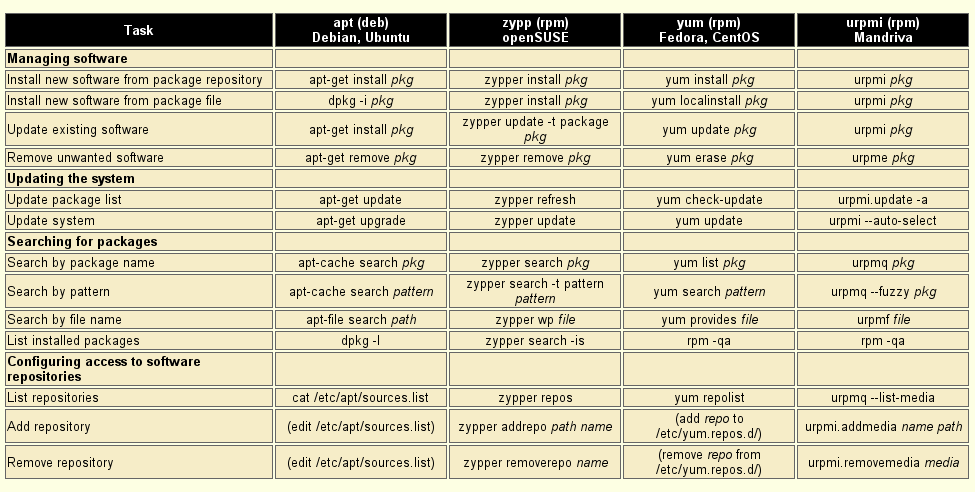
\includegraphics[scale=0.5]{src/package_managers_1.png}
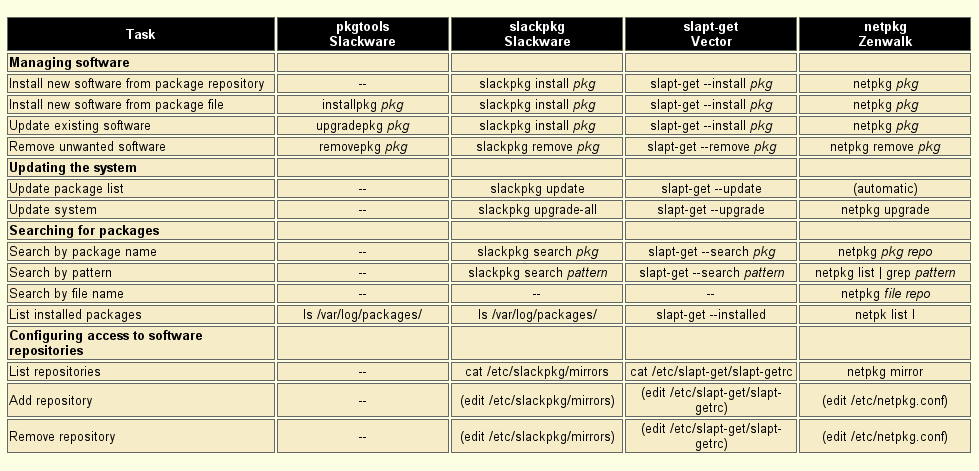
\includegraphics[scale=0.5]{src/package_managers_2.png}
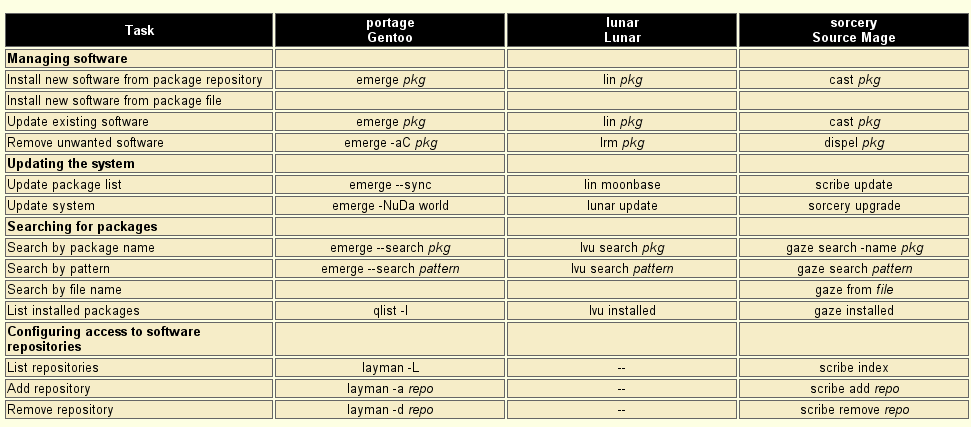
\includegraphics[scale=0.5]{src/package_managers_3.png}
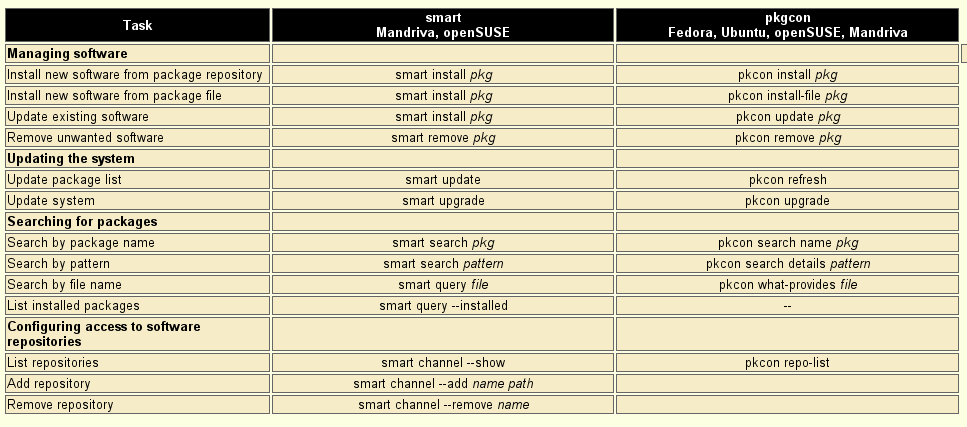
\includegraphics[scale=0.5]{src/package_managers_4.png}
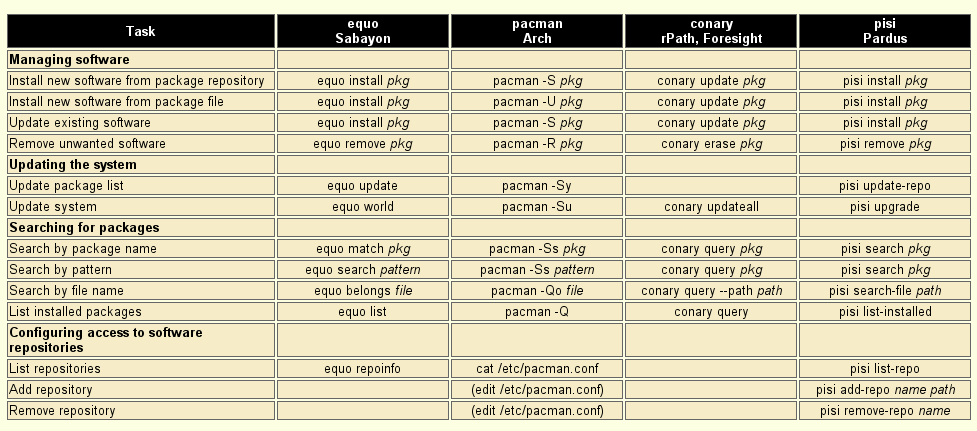
\includegraphics[scale=0.5]{src/package_managers_5.png}
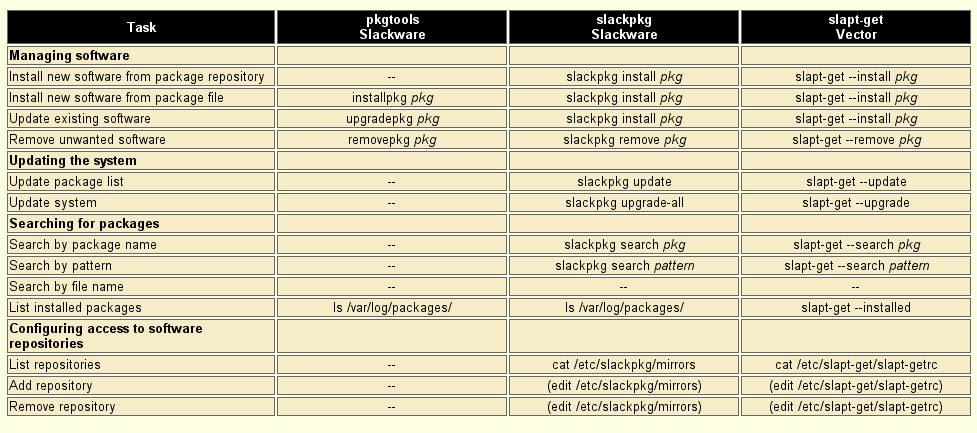
\includegraphics[scale=0.5]{src/package_managers_6.png}
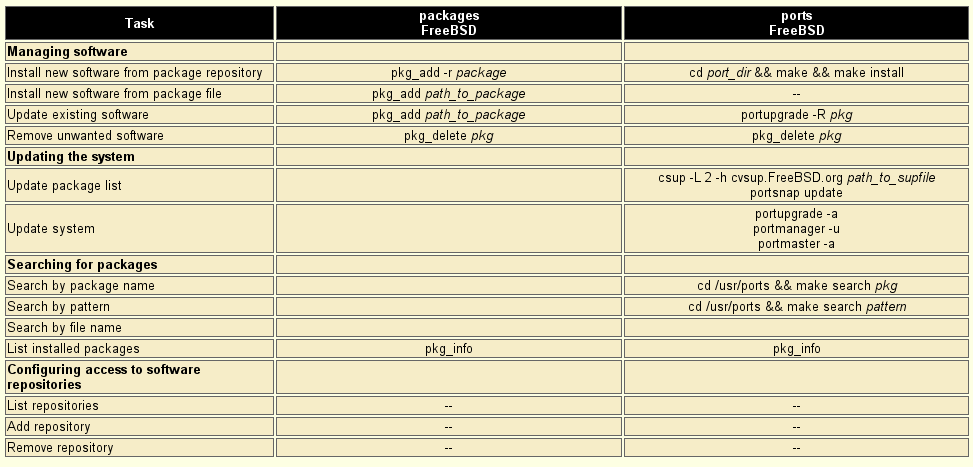
\includegraphics[scale=0.5]{src/package_managers_7.png}
\end{center}

\chapter{Creative Commons}
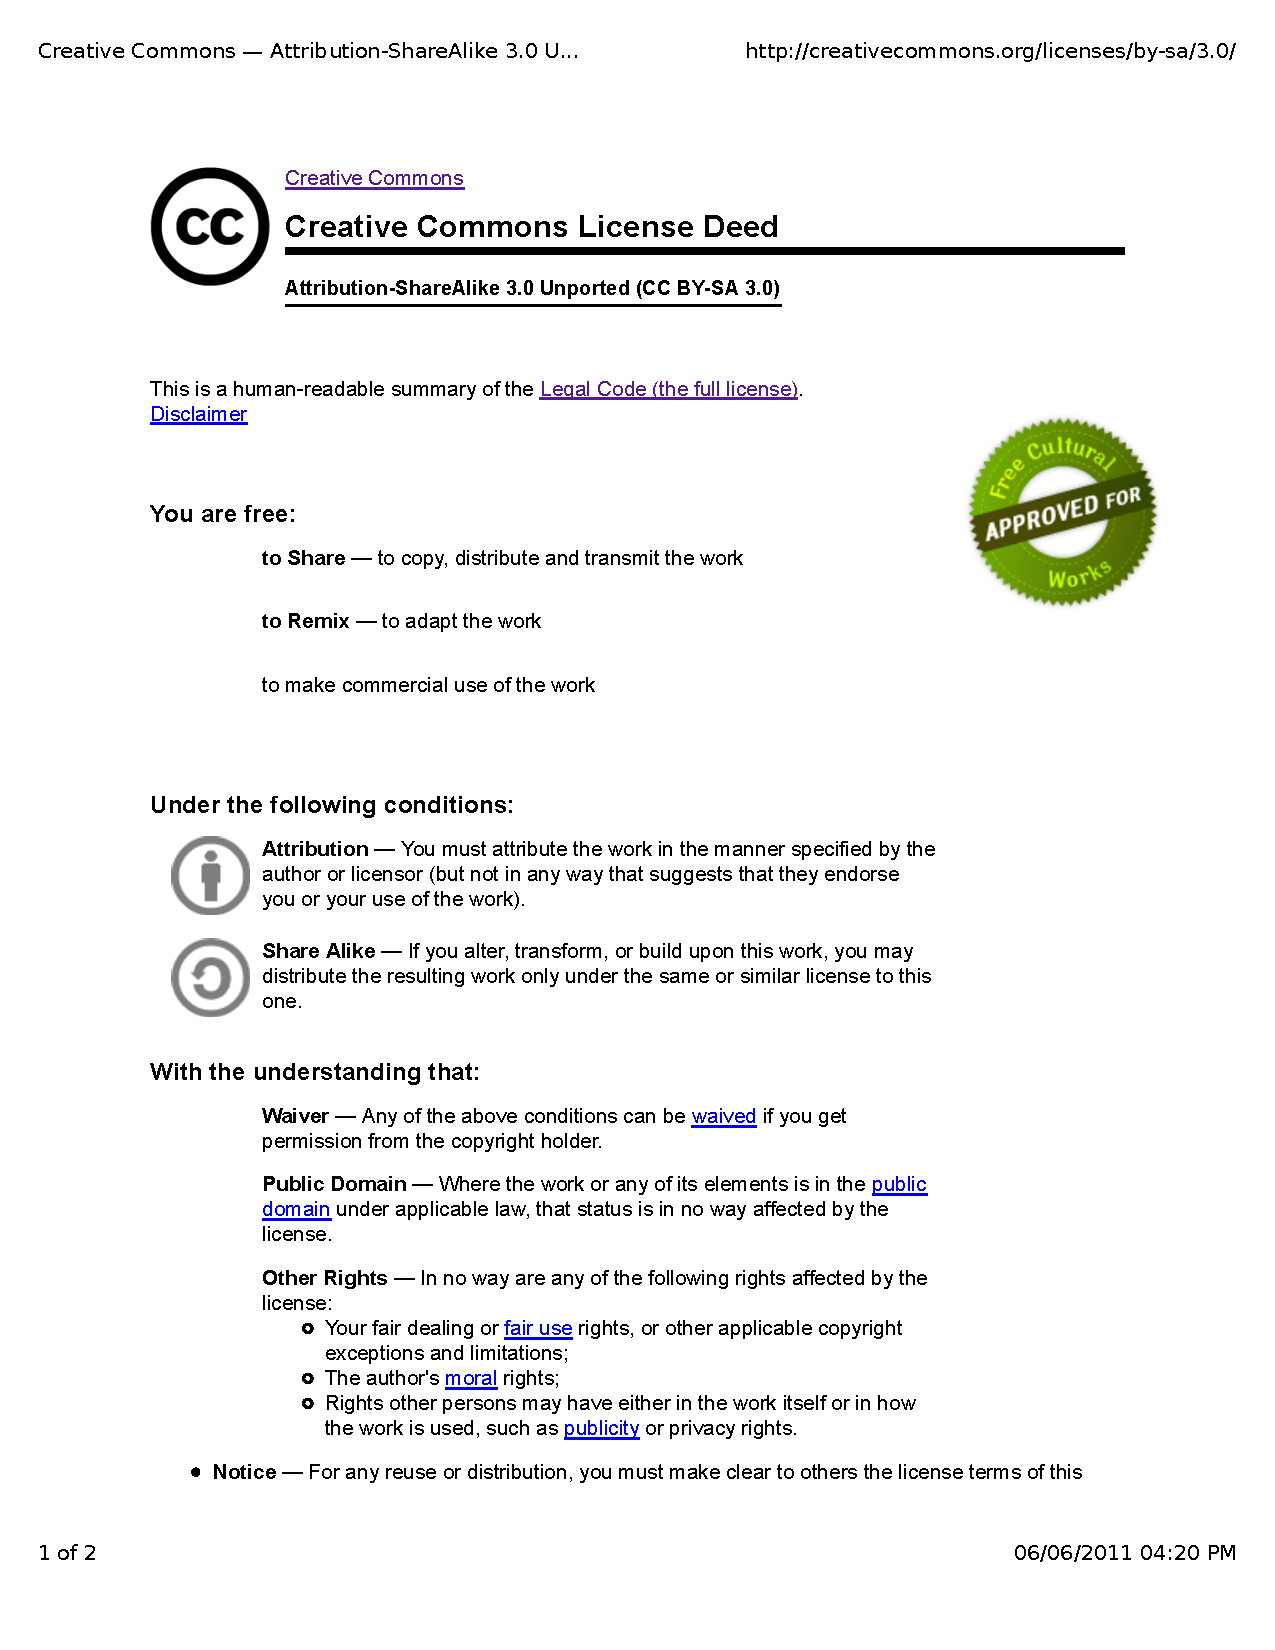
\includegraphics[scale=0.6]{src/cc-by-sa.pdf}

\chapter{UNIX bestandsrechten}
UNIX bestandsrechten zijn een grote bron van verwarring voor mensen die net beginnen met UNIX of op UNIX gelijkende besturingssytemen. In feite is het een simpel doch krachtig systeem. Bekijk even deze figuur:\\\\
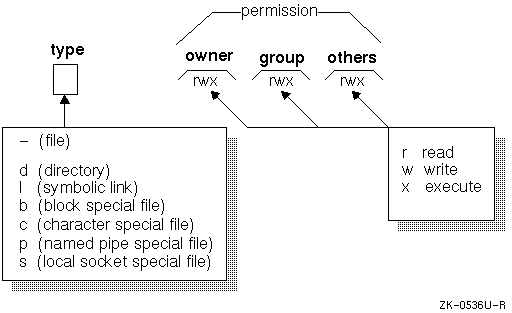
\includegraphics[scale=0.7]{src/unix_file_permissions.png}
%
Hierop zie je dat deze rechten steeds worden uitgedrukt in de vorm: 'drwxrwxrwx'. Dit kan je opdelen in een aantal verschillende stukken, namelijk: 'd rwx rwx rwx'. Hier zie je al een duidelijk onderscheid tussen de indicatie van het type bestand en de rechten die eraan worden toegewezen. Het eerste symbool (in dit geval een 'd') duidt aan wat voor type bestand je mee te maken hebt. Indien dit leeg is kan je ervan uitgaan dat je te maken hebt met een gewoon bestand. Indien je hier een 'd' tegenkomt, duidt dit erop dat het object een map is. Andere mogelijke symbolen die je waarschijnlijk niet zo vaak zal tegenkomen zijn: 'l' voor links, 'b' voor een 'block special file', 'c' voor een 'character special file', 'p' voor een 'named pipe special file' en 's' voor een 'local socket special file'. Zoals je al kon raden zijn dit veelal uitzonderingen. In de meeste gevallen zul je enkel gewone bestanden, mappen en links tegenkomen.\\\\
%
Daarnaast hebben we de 'rwx rwx rwx' structuur. Deze is in feite drie maal hetzelfde, maar geldt voor verschillende personen of groepen. De eerste iteratie duid de rechten van de eigenaar aan, de tweede iteratie is representatief voor de groep waaraan het bestand toehoort en de derde iteratie is voor publieke toegang (iedereen die niet tot \'e\'en van voorgaande groepen behoort).\\\\
De rechten zelf worden uitgedrukt in de vorm 'rwx', wat staat voor: lezen ('r'), schrijven ('w') en uitvoeren ('x'). Afhankelijk van de beschikbare waardes zal je het betreffende bestand kunnen lezen, schrijven en/of uitvoeren. Als je de rechten 'rw-' meekrijgt zal je dit bestand bijvoorbeeld zowel kunnen openen om te lezen, als wijzigingen aanbrengen. Bij de rechten 'r-x' zal je het bestand enkel kunnen lezen en uitvoeren. Dit zijn de permissies in hun simpelste vorm, maar deze zijn relatief lang om steeds op te schrijven. Daarom werd een systeem ontwikkeld waarbij deze rechten worden omgezet in cijfer. Zo krijg je voor elk van deze groepen \'e\'en cijfer, wat het een stuk compacter maakt. De waarde van deze cijfers is afhankelijk van de rechten die je erop bezit: 4 voor lezen, 2 voor schrijven en 1 voor uitvoeren. Dit zorgt ervoor dat er geen verwarring kan ontstaan over welke waarde wat betekend, aangezien alle waardes en combinaties van waardes uniek zijn. Indien je dus rechten hebt op zowel het lezen als schrijven van een bestand, worden jouw rechten opgeteld tot 6 (4 + 2). Indien je mag lezen en uitvoeren wordt dit 5 (4+1). De hoogst mogelijk rechten omvatten de mogelijkheid om zowel te lezen, schrijven en uitvoeren (rwx). Dit zorgt dan voor een totaal van 7 (4 + 2 + 1).\\\\
Deze rechten worden dan een 'mode' genoemd en worden uitgedrukt als een drie-cijferige waarde, waarbij de getallen respectievelijk de eigenaarsrechten, groepsrechten en publieke rechten omschrijven. Als je een bestand enkel toegankelijk wil maken voor jezelf, kan je dus een waarde opgeven van '700', wat ervoor zorgt dat je zelf alles kan doen met je bestand maar het niet toegankelijk is voor andere mensen. Een waarde van '644' zorgt er dan weer voor dat je zelf een bestand kan uitlezen en wijzigen, maar al de rest enkel het bestand kan uitlezen. 


Dit eindwerk is opgebouwd in de taal Latex\\
Dit is een typesetting taal die speciaal ontwikkeld is voor het opmaken van documenten,
met vele uitvoerformaten.\\
Het is een zeer flexibele taal met veel mogelijkheden gaande van automatische generatie van de inhoudsopgave tot het weergeven van wiskundige berekeningen met vierkantswortels ed.\\

% -----------------------------------------------


\backmatter
% -----------------------------------------------
\begin{thebibliography}{99}

\bibitem{puppetlabs}www.puppetlabs.com
\bibitem{puppetlabs coredocs}docs.puppetlabs.com/guides/style.html
\bibitem{puppetlabs guides}docs.puppetlabs.com/guides/
\bibitem{config management wiki}en.wikipedia.org/wiki/Configuration\_management

\end{thebibliography}

%\printindex
% -----------------------------------------------

\end{document}
